\documentclass[]{tufte-handout}

% ams
\usepackage{amssymb,amsmath}

\usepackage{ifxetex,ifluatex}
\usepackage{fixltx2e} % provides \textsubscript
\ifnum 0\ifxetex 1\fi\ifluatex 1\fi=0 % if pdftex
  \usepackage[T1]{fontenc}
  \usepackage[utf8]{inputenc}
\else % if luatex or xelatex
  \makeatletter
  \@ifpackageloaded{fontspec}{}{\usepackage{fontspec}}
  \makeatother
  \defaultfontfeatures{Ligatures=TeX,Scale=MatchLowercase}
  \makeatletter
  \@ifpackageloaded{soul}{
     \renewcommand\allcapsspacing[1]{{\addfontfeature{LetterSpace=15}#1}}
     \renewcommand\smallcapsspacing[1]{{\addfontfeature{LetterSpace=10}#1}}
   }{}
  \makeatother

\fi

% graphix
\usepackage{graphicx}
\setkeys{Gin}{width=\linewidth,totalheight=\textheight,keepaspectratio}

% booktabs
\usepackage{booktabs}

% url
\usepackage{url}

% hyperref
\usepackage{hyperref}

% units.
\usepackage{units}


\setcounter{secnumdepth}{-1}

% citations

\newlength{\cslhangindent}
\setlength{\cslhangindent}{1.5em}
% For Pandoc 2.8 to 2.11
\newenvironment{cslreferences}%
  {}%
  {\par}
% For pandoc 2.11+ using new --citeproc
\newlength{\csllabelwidth}
\setlength{\csllabelwidth}{3em}
\newenvironment{CSLReferences}[3] % #1 hanging-ident, #2 entry spacing
 {% don't indent paragraphs
  \setlength{\parindent}{0pt}
  % turn on hanging indent if param 1 is 1
  \ifodd #1 \everypar{\setlength{\hangindent}{\cslhangindent}}\ignorespaces\fi
  % set entry spacing
  \ifnum #2 > 0
  \setlength{\parskip}{#2\baselineskip}
  \fi
 }%
 {}
\usepackage{calc}
\newcommand{\CSLBlock}[1]{#1\hfill\break}
\newcommand{\CSLLeftMargin}[1]{\parbox[t]{\csllabelwidth}{#1}}
\newcommand{\CSLRightInline}[1]{\parbox[t]{\linewidth - \csllabelwidth}{#1}}
\newcommand{\CSLIndent}[1]{\hspace{\cslhangindent}#1}

% pandoc syntax highlighting

% table with pandoc
\usepackage{longtable,booktabs,array}
\usepackage{calc} % for calculating minipage widths
% Correct order of tables after \paragraph or \subparagraph
\usepackage{etoolbox}
\makeatletter
\patchcmd\longtable{\par}{\if@noskipsec\mbox{}\fi\par}{}{}
\makeatother
% Allow footnotes in longtable head/foot
\IfFileExists{footnotehyper.sty}{\usepackage{footnotehyper}}{\usepackage{footnote}}
\makesavenoteenv{longtable}

% multiplecol
\usepackage{multicol}

% strikeout
\usepackage[normalem]{ulem}

% morefloats
\usepackage{morefloats}


% tightlist macro required by pandoc >= 1.14
\providecommand{\tightlist}{%
  \setlength{\itemsep}{0pt}\setlength{\parskip}{0pt}}

% title / author / date
\title{97039 - GLOBAL HEALTH, ANTIMICROBIAL DRUGS AND VACCINES}
\author{Russell E. Lewis, Associate Professor, Infectious Diseases,
University of Bologna}
\date{11/26/2022}


\begin{document}

\maketitle




\hypertarget{a-brief-history-of-antimicrobial-resistance-amr}{%
\subsection*{A brief history of antimicrobial resistance
(AMR)}\label{a-brief-history-of-antimicrobial-resistance-amr}}
\addcontentsline{toc}{subsection}{A brief history of antimicrobial
resistance (AMR)}

Until the 20th Century, influenza and pneumonia, tuberculosis, and
enteric infections were among the top thee causes of death. The average
life expectancy of adults in Western Europe was less than 50 years (Fig
1), and 2\% of children failed to live beyond 5 years of age due to
deaths caused by infectious diseases.

Industrialization and growing wealth during the 19th century brought
improvements in drinking water and sanitation in many countries,
reducing communicable enteric infections and improvements in life
expectancy. By the early 20th century, advances in immunization led to
the introduction of vaccines for pertussis, diptheria, yellow fever and
tuberculosis. However, common bacterial infections remained a common
cause of death. Streptococcal throat infections were sometimes fatal,
ear infections could lead to deafness, mastoiditis or meningitis with a
90\% mortality rate, and surgery or childbirth was associated with high
complication rates and frequent maternal deaths.

Figure 1. Changes in life expectancy over 500 years. Data source: World
Health Bank

Bacteria and mechanisms of bacterial resistance to natural metabolites
produces by other bacteria nad fungi have existed for over 2-2.5 billion
years. In contrast, it is estimated that that first humans emerged 2
million years ago. While products with antimicrobial activity had been
used as medicines for millennia to treat infections, the causes of
infection were not known until the 19th and 20th centuries. Therefore,
it cannot be said that humans are the cause of antimicrobial resistance.

The microbiologist and immunologist Paul Erlich (1854-1915) is credited
with the discovery and first medical application of a synthetic
antibiotic arsphenamine (Salvarsan) in the treatment of bacterial
infection- syphilis. However, it was the serendipitous discovery of
penicillin on September 3, 1928 by Alexander Fleming, and its subsequent
purification of the drug in quantities needed for clinical testing in
humans by Drs. Florey and Chain in the late 1930s, that lead to the
major breakthrough of antibiotic treatment for common bacterial
infections. Alexander Fleming was also among the first physicians to
caution about the risks of resistance to penicillin if used too little
or for a too short of period during treatment.

\begin{quote}
``It is not difficult to make microbes resistant to penicillin in the
laboratory by exposing them to concentrations not sufficient to kill
them, and the same thing has occasionally happened in the body. The time
may come when penicillin can be bought by anyone in the shops. Then
there is the danger that the ignorant man may easily under-dose himself
and by exposing his microbes to non-lethal quantities of the drug make
them resistant.'' -Sir Alexander Fleming, Nobel Prize Lecture, December
11, 1945
\end{quote}

By 1947, Fleming's predictions were realized as the first cases of
penicillin resistance reported. Thus began the ``arms race'' between the
``emergence'' and spread of new antimicrobial resistance mechanisms and
discovery of new antibiotics to treat these resistant pathogens.
Initially, antibiotic discovery seemed to keep pace with resistance as a
host of new chemical classes were developed and introduced in the
1950s-1980's. During this time, it was often possible to simply switch
treatment once resistance against a specific antibiotic became a major
problem. By the 1980's the discovery of new agents began to slow (Fig
2). The latest discovery of a new antibiotic class that has reached the
market was in 1987. Since then, there has been a lack of innovation in
the field, and today there are few novel antibiotic classes in the drug
pipeline. In Module 2 we will examine the scientific challenges and
market forces that have made new antibiotic discovery increasingly
difficult and how access to newer antibiotics is limited in many parts
of the world.

Once resistance has developed, it can spread from a colonised patient to
another patient if appropriate hygienic precautions (e.g., hand hygiene,
isolation) are not taken. The risk of resistant bacteria spreading is
amplified in crowded environments, especially when people in the
surrounding area are receiving antibiotics - a common situation in
hospitals and other healthcare facilities.

The consequences of faltering antibiotic discovery are now seen
worldwide as more and more bacterial infections are becoming harder to
treat again. Especially worrisome is the lack of antibiotics against
Gram-negative bacteria. The rapid global spread of multi- and
pan-resistant bacteria, also known in the lay press as ``superbugs,''
can cause infections that are not treatable with existing antibiotics.

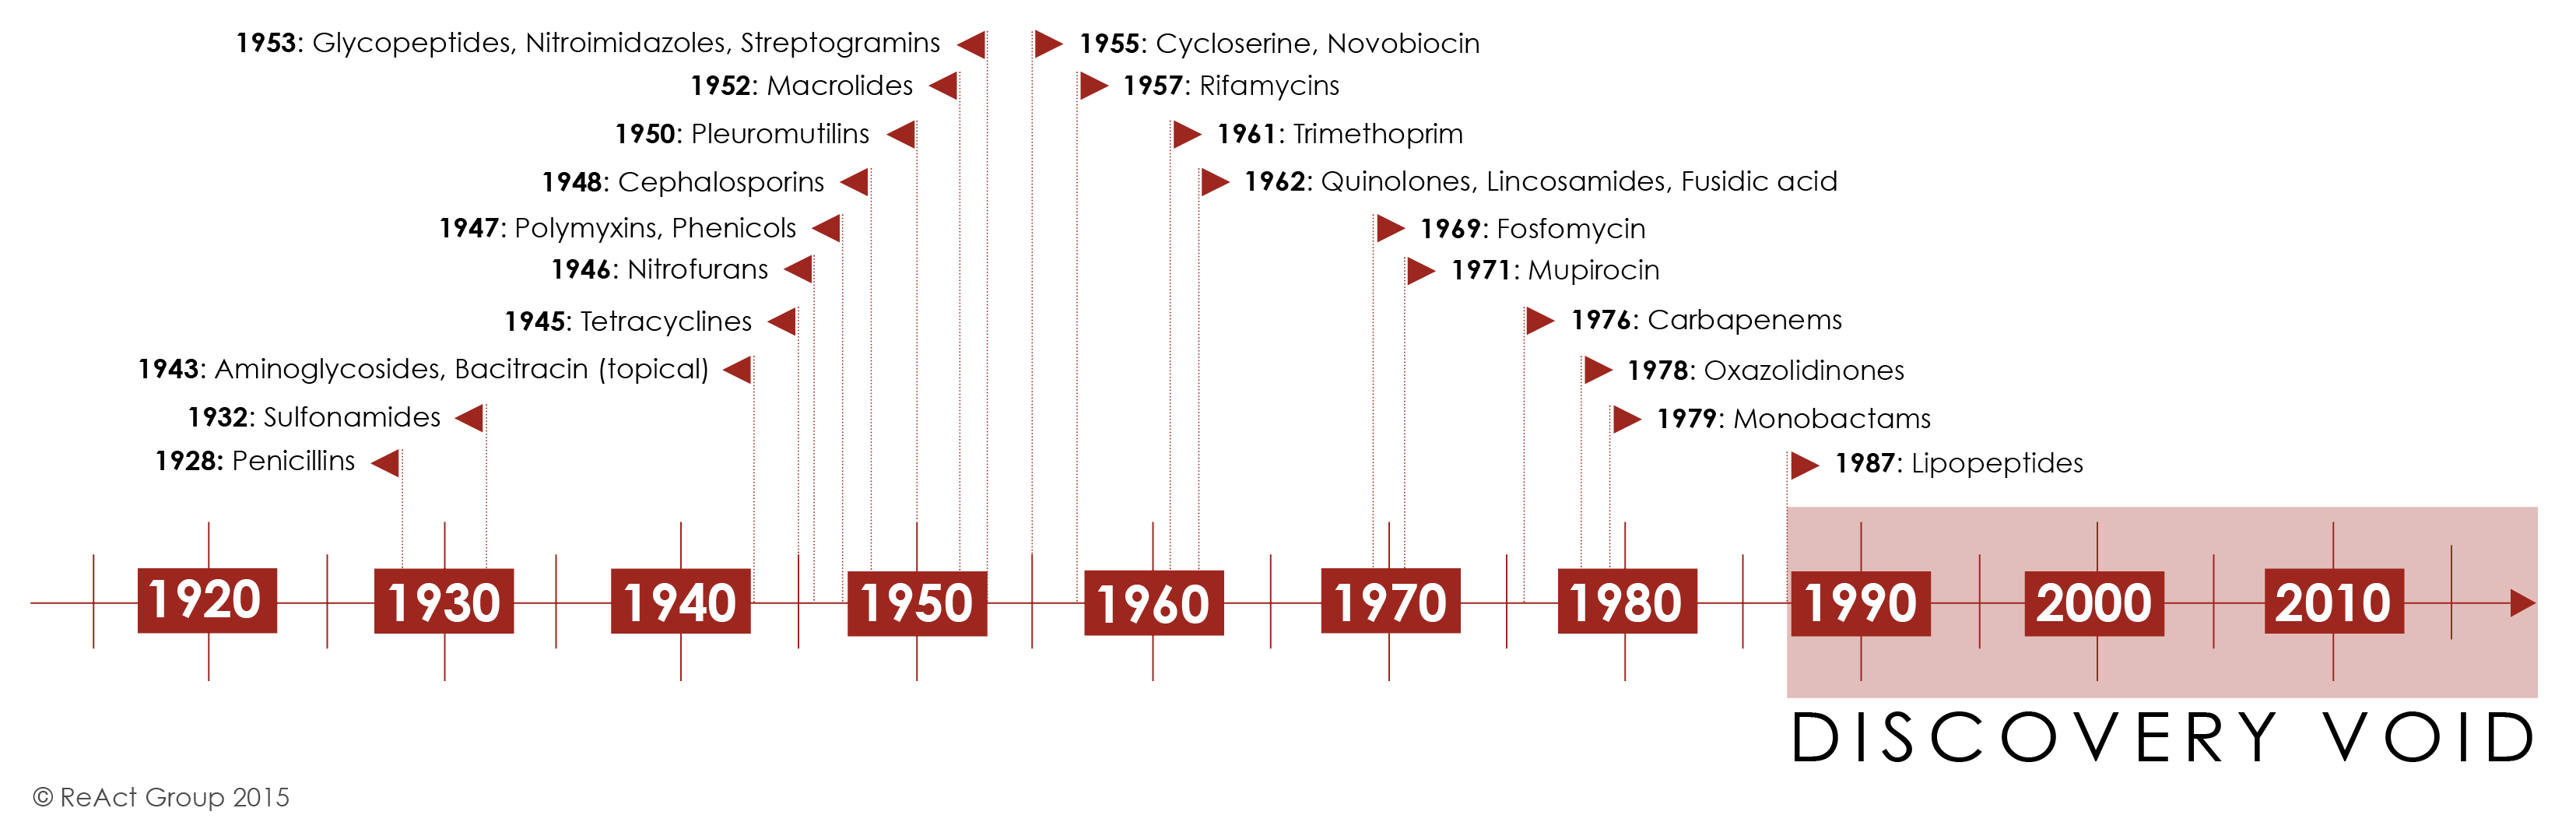
\includegraphics[width=16.66667in,height=\textheight]{images/ab-discovery-timeline.png}

Figure 2. Antibiotic discovery timeline. Source ReACT Group 2015.

Recognizing the growing global threat of antibiotic resistance (AMR) on
human health but also the economy and human development, The World
Health Organization (WHO) and World Organisation for Animal Health (OIE)
proposed as a
\href{https://www.who.int/publications/i/item/9789241509763}{Global
Action Plan for AMR} in 2017 and more recently a
\href{https://www.who.int/news/item/30-07-2021-call-to-action-on-antimicrobial-resistance-2021}{``Call
to Action on Antimicrobial Resistance''} in 2021. The plan outlines 21
strategies and 5 strategic objectives action plans that should be
implemented in member states to address AMR. These include:

\begin{enumerate}
\def\labelenumi{\arabic{enumi}.}
\tightlist
\item
  Improvements in the awareness and understanding of antimicrobial
  resistance through effective communication, education and training
\item
  Strengthening of knowledge and evidence base of AMR through
  surveillance and research
\item
  Reductions in the incidence of infection through effective sanitation,
  hygiene and infection prevention measures
\item
  Optimization the use of antimicrobial medicines in human and animal
  health
\item
  Development of an economic case for sustainable investment in AMR
  research that takes account of the needs of all countries, and
  increase investment in new medicines, diagnostic tools, vaccines and
  other interventions
\end{enumerate}

The WHO also published a
\href{https://www.who.int/medicines/publications/WHO-PPL-Short_Summary_25Feb-ET_NM_WHO.pdf}{Priority
Pathogen List} for research and development of new antibiotics (Table
1). This priority list includes bacterial pathogens that are considered
to be be the biggest threat to human health in addition to
\emph{Mycobacterium tuberculosis.} The WHO list breaks down pathogens
into three groups:

Table 1. WHO priority pathogens

\begin{longtable}[]{@{}
  >{\raggedright\arraybackslash}p{(\columnwidth - 2\tabcolsep) * \real{0.1622}}
  >{\raggedright\arraybackslash}p{(\columnwidth - 2\tabcolsep) * \real{0.8378}}@{}}
\toprule
\begin{minipage}[b]{\linewidth}\raggedright
Priority
\end{minipage} & \begin{minipage}[b]{\linewidth}\raggedright
Pathogens included
\end{minipage} \\
\midrule
\endhead
\textbf{Critical} & \emph{Acinetobacter baumannii}
(Carbapenem-resistant)

\emph{Pseudomonas aeruginosa} (Carbapenem-resistant)

Enterbacterales (3rd generation cephalosporin, carbapenem-resistant) \\
\textbf{High} & \emph{Enterococcus faecium}, vancomycin-resistant

\emph{Staphylococcus aureus}, methicillin-resistant, vancomycin
intermediate and resistant

\emph{Helicobacter pylori}, clarithromycin-resistant

\emph{Campylobacter}, fluoroquinolone-resistant

\emph{Salmonella} spp., fluoroquinolone-resistant

\emph{Neisseria gonorrhoeae}, 3rd generation cephalosporin-resistant,
fluoroquinolone-resistant \\
\textbf{Medium} & \emph{Streptococcus pneumoniae},
penicillin-non-susceptible

\emph{Haemophilus influenzae}, ampicillin-resistant

\emph{Shigella} spp., fluoroquinolone-resistant \\
\bottomrule
\end{longtable}

These pathogens may exhibit multi-drug resistance (MDR),\footnote{MDR-
  resistance to one agent in at least 3 antibiotic categories; XDR-
  resistant except to 2 or fewer antibiotic categories; PDR- resistant
  to all agents in all antibiotic categories; DTR-requires the use of
  less-effective or more toxic ``reserve'' antibiotics} extensive drug
resistance (XDR) or pan-drug resistance (PDR)(Magiorakos et al. 2012).
Difficult-to-treat resistance (DTR) is a newer definition used to define
isolate resistance patterns that require the use of less-effective or
more toxic ``reserve'' antibiotics- e.g., \emph{Acinetobacter baumanii}
susceptible only to colistin and tobramycin (Kadri et al. 2018).

Currently, both the
\href{https://apps.who.int/iris/bitstream/handle/10665/312266/9789241515528-eng.pdf}{WHO}
and
\href{https://www.oie.int/en/what-we-do/global-initiatives/antimicrobial-resistance/\#ui-id-4}{OIE}
have also developed lists of antibiotics that are considered of
``critical importance'' for human and animal medicine. These lists help
establish priorities for antimicrobial resistance surveillance and new
drug development.

\hypertarget{what-are-the-drivers-of-antimicrobial-resistance}{%
\subsection*{What are the drivers of antimicrobial
resistance?}\label{what-are-the-drivers-of-antimicrobial-resistance}}
\addcontentsline{toc}{subsection}{What are the drivers of antimicrobial
resistance?}

AMR is a natural phenomenon. Most antimicrobial drugs are naturally
produced by micro-organisms, including environmental fungi and
saprophytic bacteria, or are synthetic modifications of these natural
products, with only a few drugs (e.g., sulphonamides and
fluoroquinolones) being wholly synthetic. Yet AMR selection is
accelerated by antimicrobial exposure in health care, agriculture, and
the environment. Further transmission is affected by standards of
infection control in healthcare settings, sanitation, access to clean
water, access to assured quality antimicrobials and diagnostics, travel,
and migration (Fig 3).

Antimicrobials are among the most commonly prescribed drugs used in
human medicine, yet up to 50\% of all antimicrobials prescribed to
people are considered unnecessary. This use, misuse, or overuse of
antimicrobial drugs is considered to be a major driving force towards
antimicrobial resistance.

In human beings, the concentration of antibiotic prescribing might be
highest in inpatient settings, with 30--40\% of patients on antibiotics
in European hospitals. However, the overall highest \emph{quantity} of
antimicrobial prescribing is highest in the community setting.

More antimicrobials are used in food production than in human beings,
with marked national differences in the number of antimicrobial drugs
used in food producing animals. Various studies have shown that
antimicrobial resistance has, at least in part, emerged as a result of
the selective pressure exerted by antimicrobial use outside of human
medicine, namely in veterinary medicine, food-animal and fish
production, and agriculture

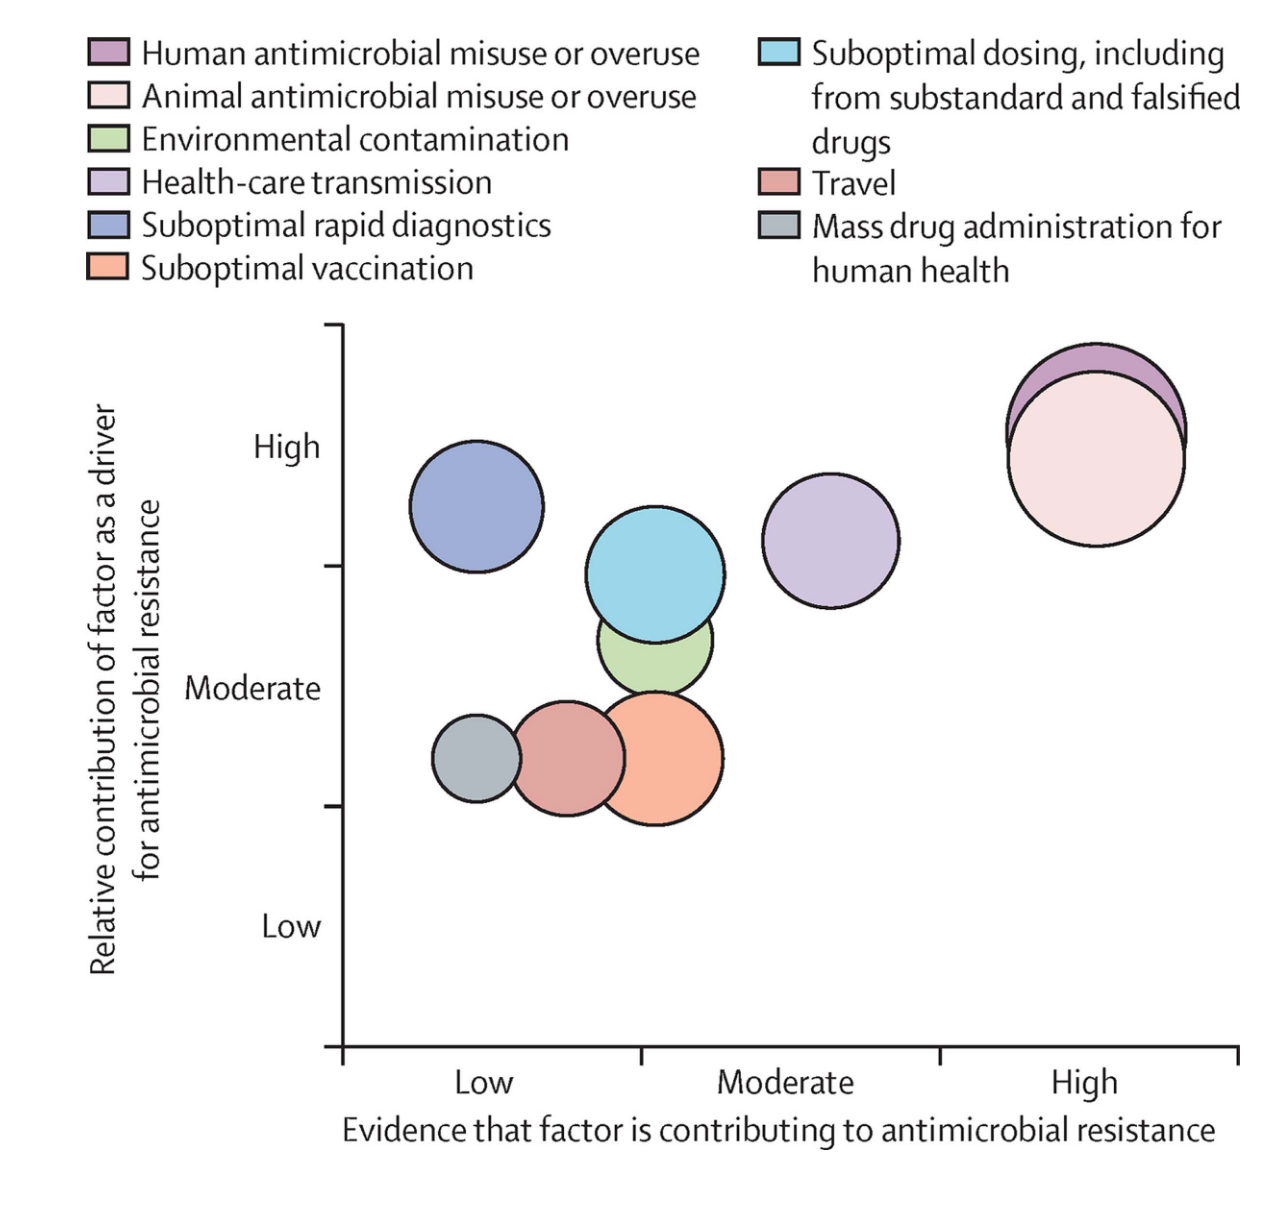
\includegraphics[width=5.20833in,height=\textheight]{images/modifiablerisk.png}

Figure 3. Modifiable risk factors that drive antimicrobial resistance.
Figure from reference (Holmes et al. 2016)

\hypertarget{how-can-antimicrobials-be-used-to-preserve-their-effectiveness-and-delay-resistance-in-humans}{%
\subsubsection*{How can antimicrobials be used to preserve their
effectiveness and delay resistance in
humans?}\label{how-can-antimicrobials-be-used-to-preserve-their-effectiveness-and-delay-resistance-in-humans}}
\addcontentsline{toc}{subsubsection}{How can antimicrobials be used to
preserve their effectiveness and delay resistance in humans?}

Strategies for the prevention and containment of AMR frequently focus
on:

\begin{enumerate}
\def\labelenumi{\arabic{enumi}.}
\tightlist
\item
  Improvement of infection diagnosis and prescription practices
  (antimicrobial stewardship)
\item
  Reduction of antimicrobial use in agriculture and environmental
  exposure in general
\item
  Development of new antimicrobials
\item
  Access to essential medicines of assured quality
\item
  Improvement of AMR surveillance
\end{enumerate}

Antimicrobial stewardship is a coordinated program that promotes and
focuses on the appropriate use of antimicrobials (including
antibiotics), improves patient outcomes, reduces microbial resistance,
and decreases the spread of infections caused by multidrug-resistant
organisms. These programs may be implemented through the use of
institution-specific treatment guidelines and an antibiotic stewardship
team (typically infectious diseases physicians with a clinical
pharmacist) who carry out full-time activities to promote and encourage
appropriate antibiotic use. While these programs have been shown to be
successful, many gaps remain in the knowledge of how to optimally design
and sustain stewardship programs in the hospital, and such programs are
rarely implemented outside of the hospital where most antibiotic
prescribing takes place.

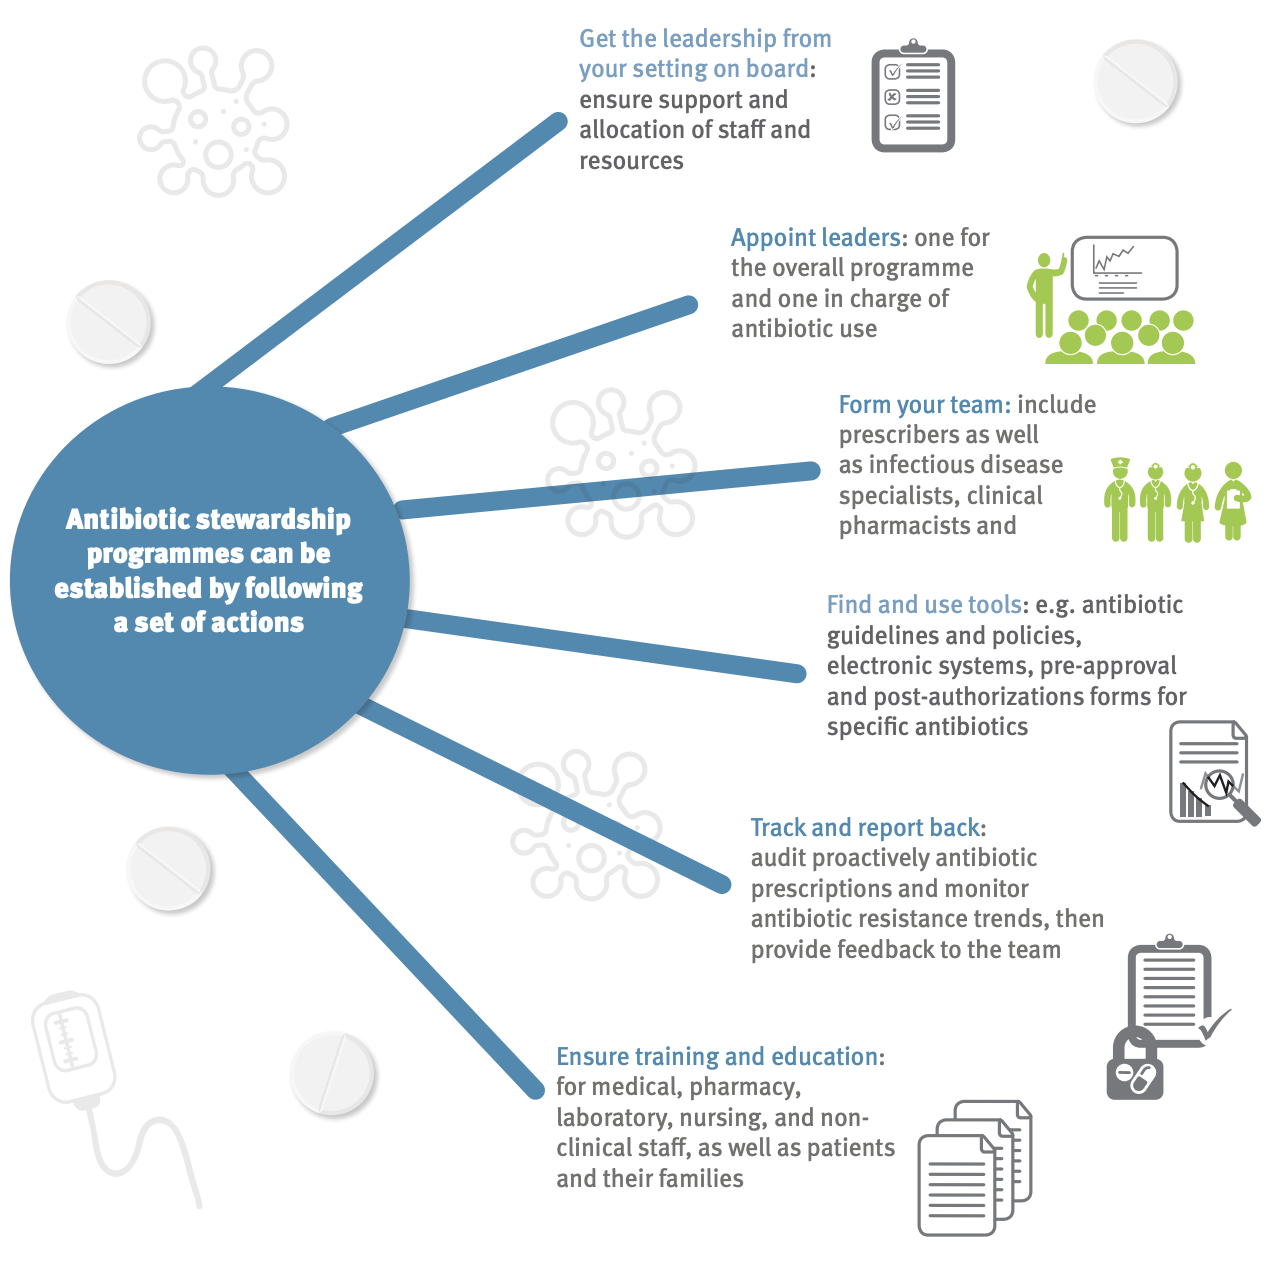
\includegraphics{images/stewardship actions.png}

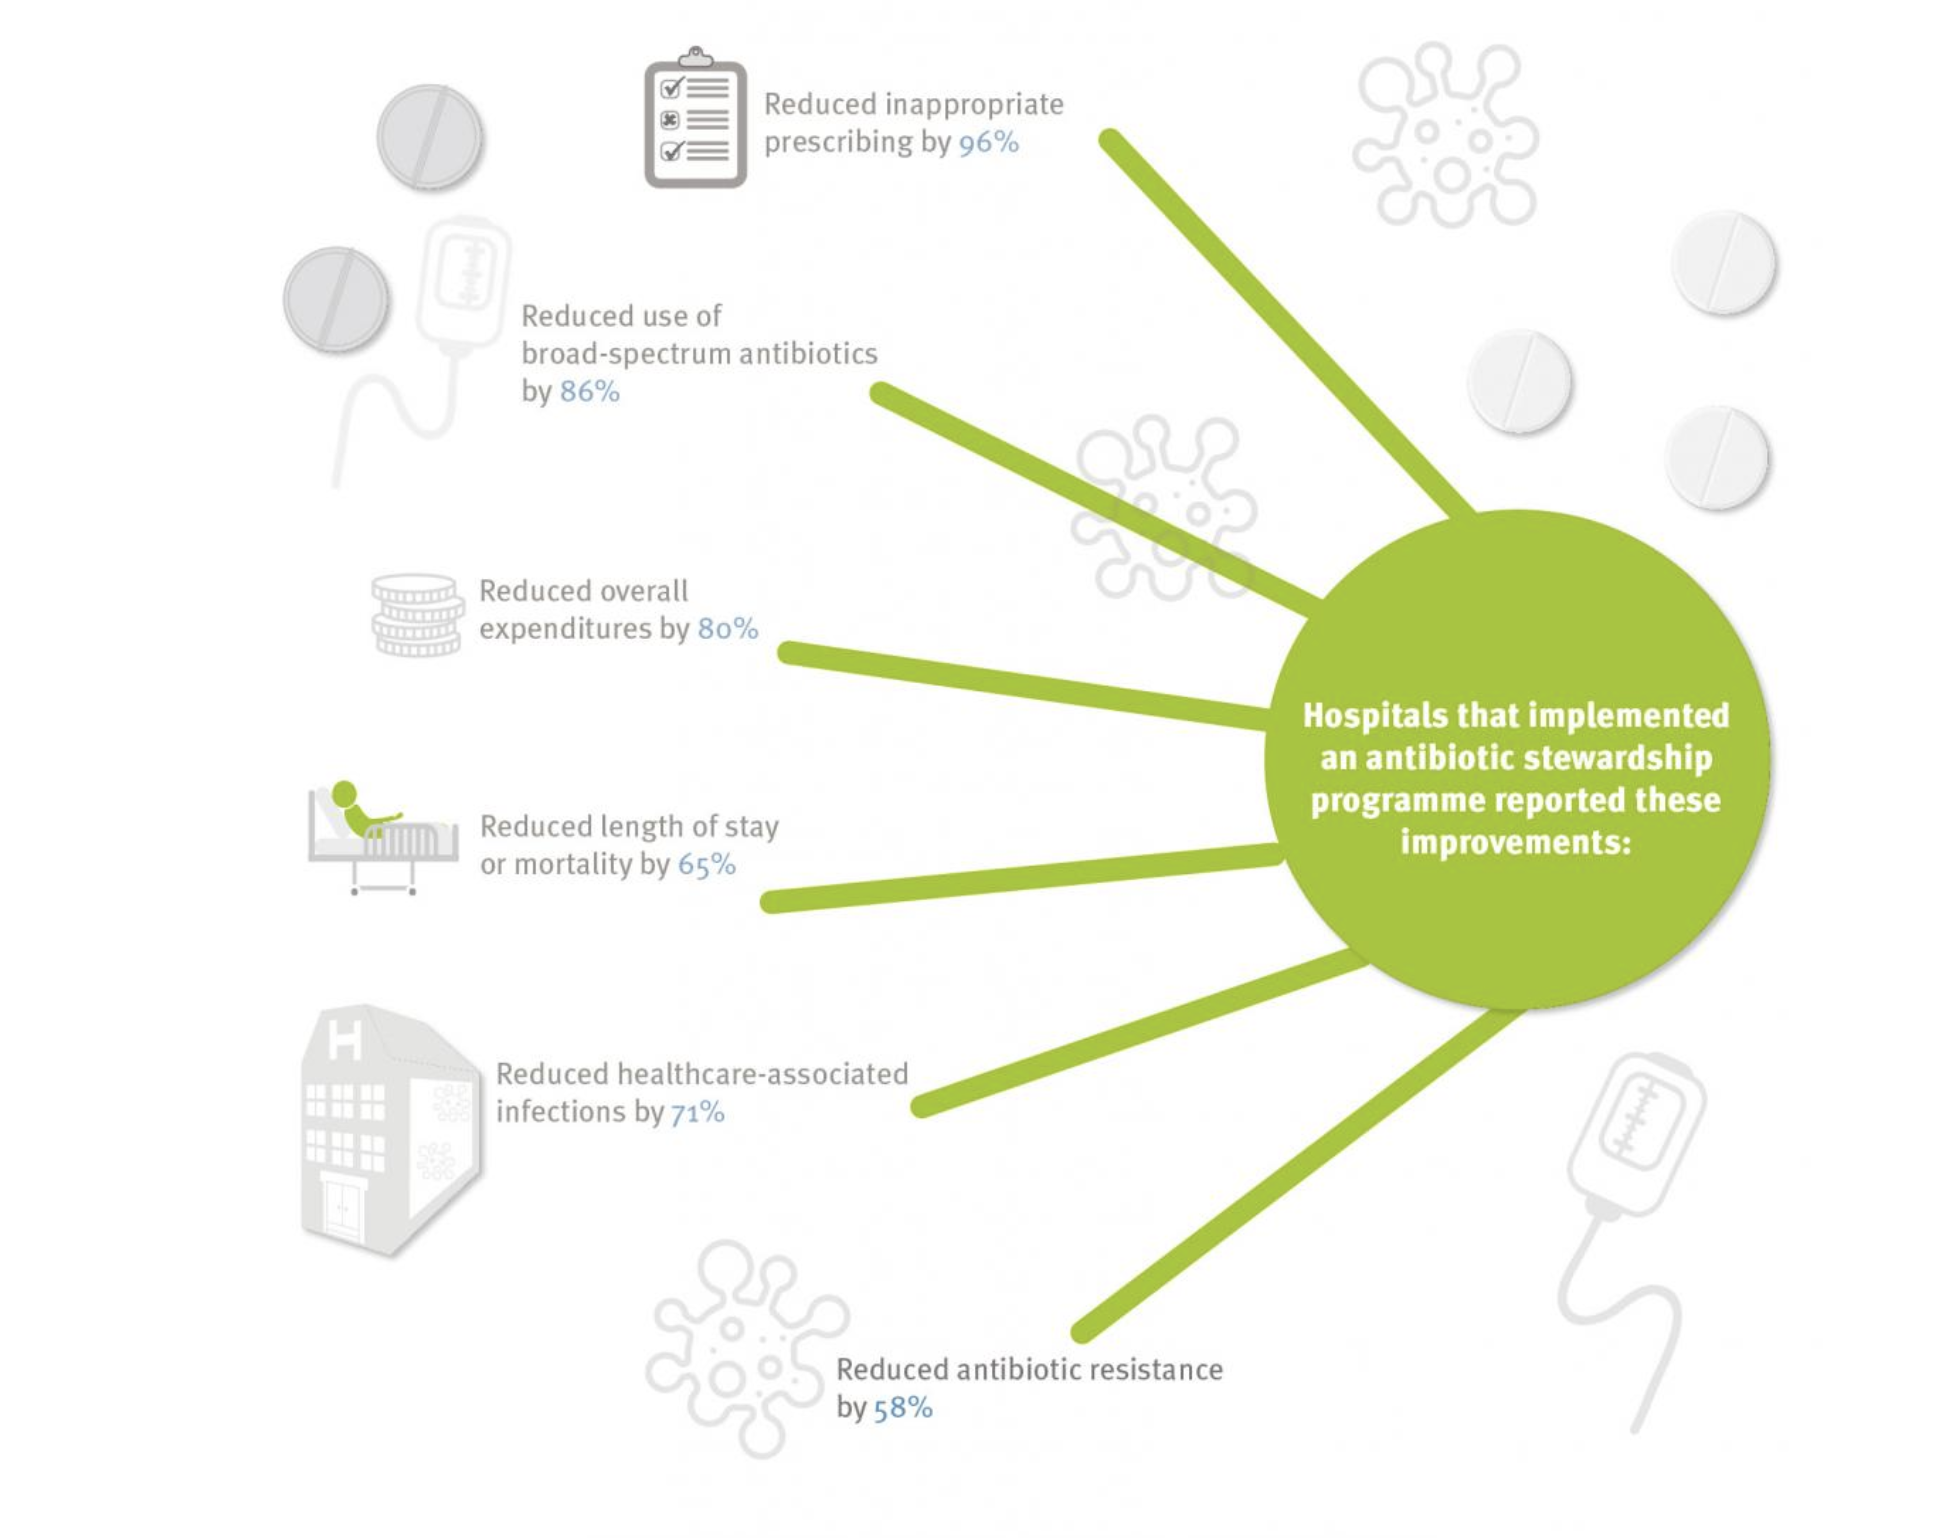
\includegraphics{images/stewardship_impl.png}

Figure 4. Examples of antimicrobial stewardship efforts and outcomes.
Source:
\href{https://antibiotic.ecdc.europa.eu/en/infographics-about-antibiotic-stewardship-programmes}{ECDC}

\hypertarget{amr-situation-in-italy}{%
\subsection*{AMR situation in Italy}\label{amr-situation-in-italy}}
\addcontentsline{toc}{subsection}{AMR situation in Italy}

Southern Europe, including Italy, has among the highest rates of
resistance for pathogens included on the WHO Priority Pathogen list. For
example, surveillance data from the European Centres for Disease Control
(ECDC) have reported a dramatic increase in multidrug-resistance (MDR)
in Italy since 2009, with now more than one-third of \emph{Klebsiella
pneumoniae} resistant to previously-considered last-line antibiotics
such as carbapenems (Fig 1.4). The link to interactive ECDC resistance
atlas can be found
\href{https://atlas.ecdc.europa.eu/public/index.aspx?Dataset=27\&HealthTopic=4}{here}.
Similarly, the Italian
\href{https://www.epicentro.iss.it/antibiotico-resistenza/epidemiologia-italia}{Micronet
Resistance Surveillance}) program has reported:

\begin{itemize}
\tightlist
\item
  26.4\% of \emph{Escherichia coli} are resistant to 3rd generation
  cephalosporins
\item
  29.5\% of \emph{Klebsiella pneumoniae} are resistant to carbapenems
  (including 33.1\% resistant to multiple drug classes)
\item
  15.9\% of \emph{Pseudomonas aeruginosa} are resistant to carbapenems
\item
  80.8\% of \emph{Acinetobacter} spp. are resistant to carbapenems with
  78.8\% of species resistant to multiple drug classes
\item
  For the Gram-positive organism \emph{Staphylococcus aureus}, the
  percentage of methicillin-resistant isolates (MRSA) remained stable,
  around 34\%, while a worrying trend continues to increase in the
  percentage of \emph{Enterococcus faecium isolates} resistant to
  vancomycin, which in 2020 was equal at 23.6\%
\item
  For \emph{Streptococcus pneumoniae} there was a slight increase in
  both the percentage of isolates resistant to penicillin (13.6\%) and
  those resistant to erythromycin (24.5\%).
\item
  Overall, higher antimicrobial resistance rates (around 40\%) are
  observed in ICUs versus general medical wards for both
  carbapenem-resistant \emph{K. pneumoniae} and methicillin-resistant
  \emph{S. aureus}.
\end{itemize}

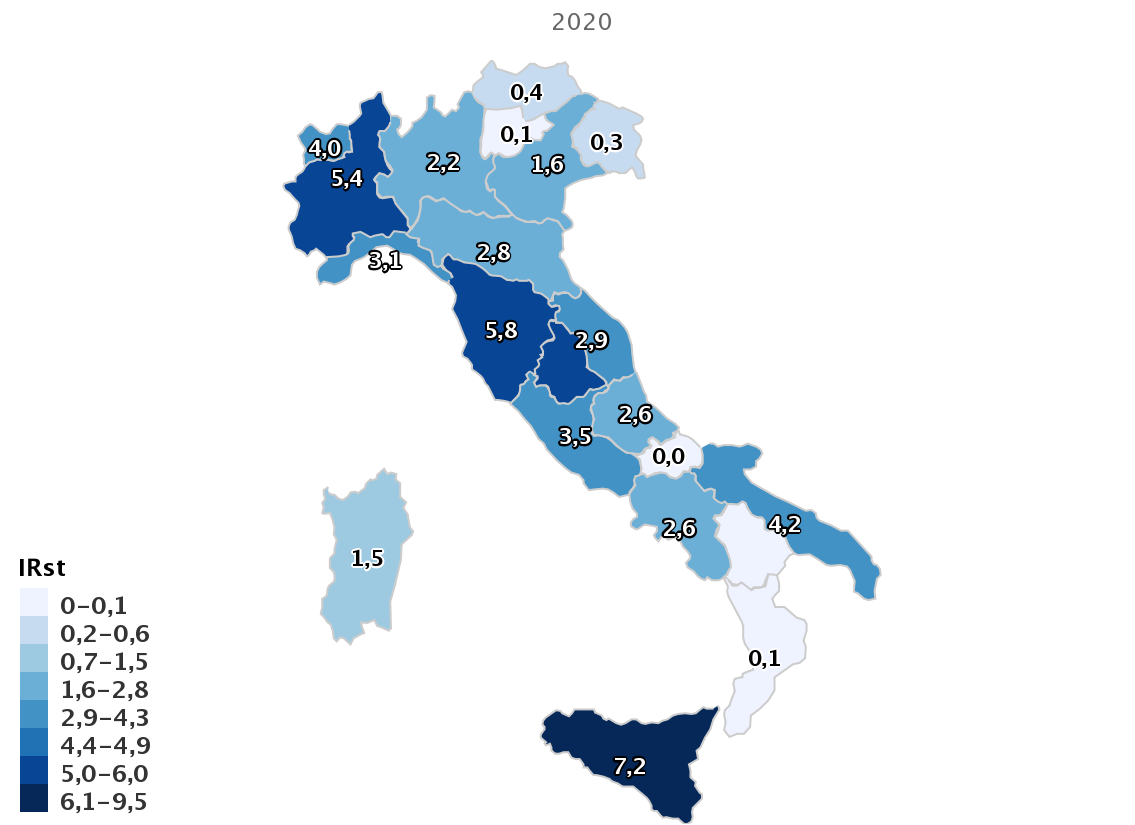
\includegraphics[width=5.20833in,height=\textheight]{images/Italia_CRE.png}

Figure 4. Regional differences in carbapenem-resistant Enterobacterales
(CRE) bloodstream infection- 2020 incidence per 100,000 residents in
Italy. Source Micronet Resistance Surveillance Program

In 2017, a
\href{https://www.ecdc.europa.eu/en/publications-data/ecdc-country-visit-italy-discuss-antimicrobial-resistance-issues}{report}
by the the ECDC noted that the AMR situation in Italian hospitals and
regions poses a major public health threat to the country. The levels of
carbapenem-resistant Enterobacteriaceae (Enterobacterales) (CRE) and
\emph{Acinetobacter baumannii} have now reached hyper-endemic levels in
many hospitals. Together with increasing methicillin-resistance among
the Gram-positive species \emph{Staphylococcus aureus} (MRSA), these
resistance trends has led to Italy's ranking as one of the Member States
with one of the highest level of antibiotic resistance in Europe.
Factors noted by the ECDC that contributed negatively to the poor
control of antibiotic resistance in Italy include:

\begin{itemize}
\tightlist
\item
  Little sense of urgency about the current AMR situation from most
  stakeholders and a tendency by many stakeholders to avoid taking
  charge of the problem
\item
  Lack of institutional support at national, regional and local level
\item
  Lack of professional leadership at each level
\item
  Lack of accountability at each level
\item
  Lack of coordination of the activities between and within levels.
\end{itemize}

\hypertarget{the-future-of-amr}{%
\subsection*{The future of AMR}\label{the-future-of-amr}}
\addcontentsline{toc}{subsection}{The future of AMR}

\begin{itemize}
\tightlist
\item
  Drug-resistant diseases already cause at least 700,000 deaths globally
  a year, including 230,000 deaths from multidrug-resistant
  tuberculosis. The estimated total number of deaths due to AMR could
  climb to 10 million deaths globally per year by 2050 under current
  projections (Fig 1.4).
\item
  Increasing resistance could lead to an unthinkable future of
  untreatable infections, reversing more than a 100 years of medical
  progress. Routine medical procedures or surgery will become more
  dangerous and associated with higher complication rates.
  Immunosuppression, cancer chemotherapy and transplantations may carry
  unacceptable risk for many patients if infections cannot be
  effectively prevented and treated.
\item
  Economic and social progress in many countries will be dramatically
  impacted by increasing AMR leading to political and social
  instability. The initial short-term economic damage of uncontrolled
  antimicrobial resistance will be comparable to the shocks experienced
  during the 2008-2009 global financial crisis and result in
  dramatically-increased healthcare expenditures; reductions in food and
  feed production, reduced economic output, and
  \href{https://documents.worldbank.org/en/publication/documents-reports/documentdetail/323311493396993758/final-report}{increased
  poverty and inequality}. The economic impact of antimicrobial
  resistance is predicted to be even greater and longer lasting on
  low-and middle-income (LMIC) countries.
\end{itemize}

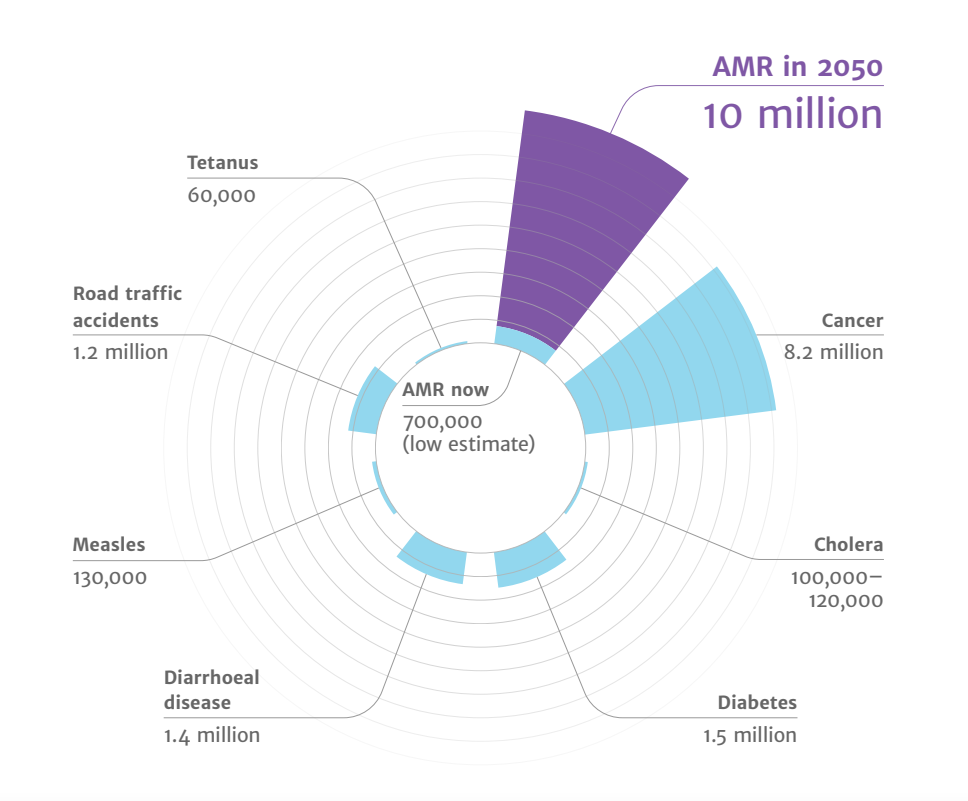
\includegraphics[width=5.20833in,height=\textheight]{images/AMR_deaths_2050.png}

Figure 5. Projected deaths due to antimicrobial resistance in 2050.
Source: O'Neil Report (O'Neill 2016).

\hypertarget{one-health-perspective-of-amr}{%
\subsection*{One-Health Perspective of
AMR}\label{one-health-perspective-of-amr}}
\addcontentsline{toc}{subsection}{One-Health Perspective of AMR}

Because the drivers of antimicrobial resistance lie in humans, animals,
plants, food and the environment, a sustained One Health response is
essential to engage and unite everyone around a shared vision and goals.
``One Health'' refers to designing and implementing programmes,
policies, legislation and research in a way that enables multiple
sectors engaged in human, terrestrial and aquatic animal and plant
health, food and feed production and the environment to communicate and
work together to achieve better public health outcomes (Fig 1.6).

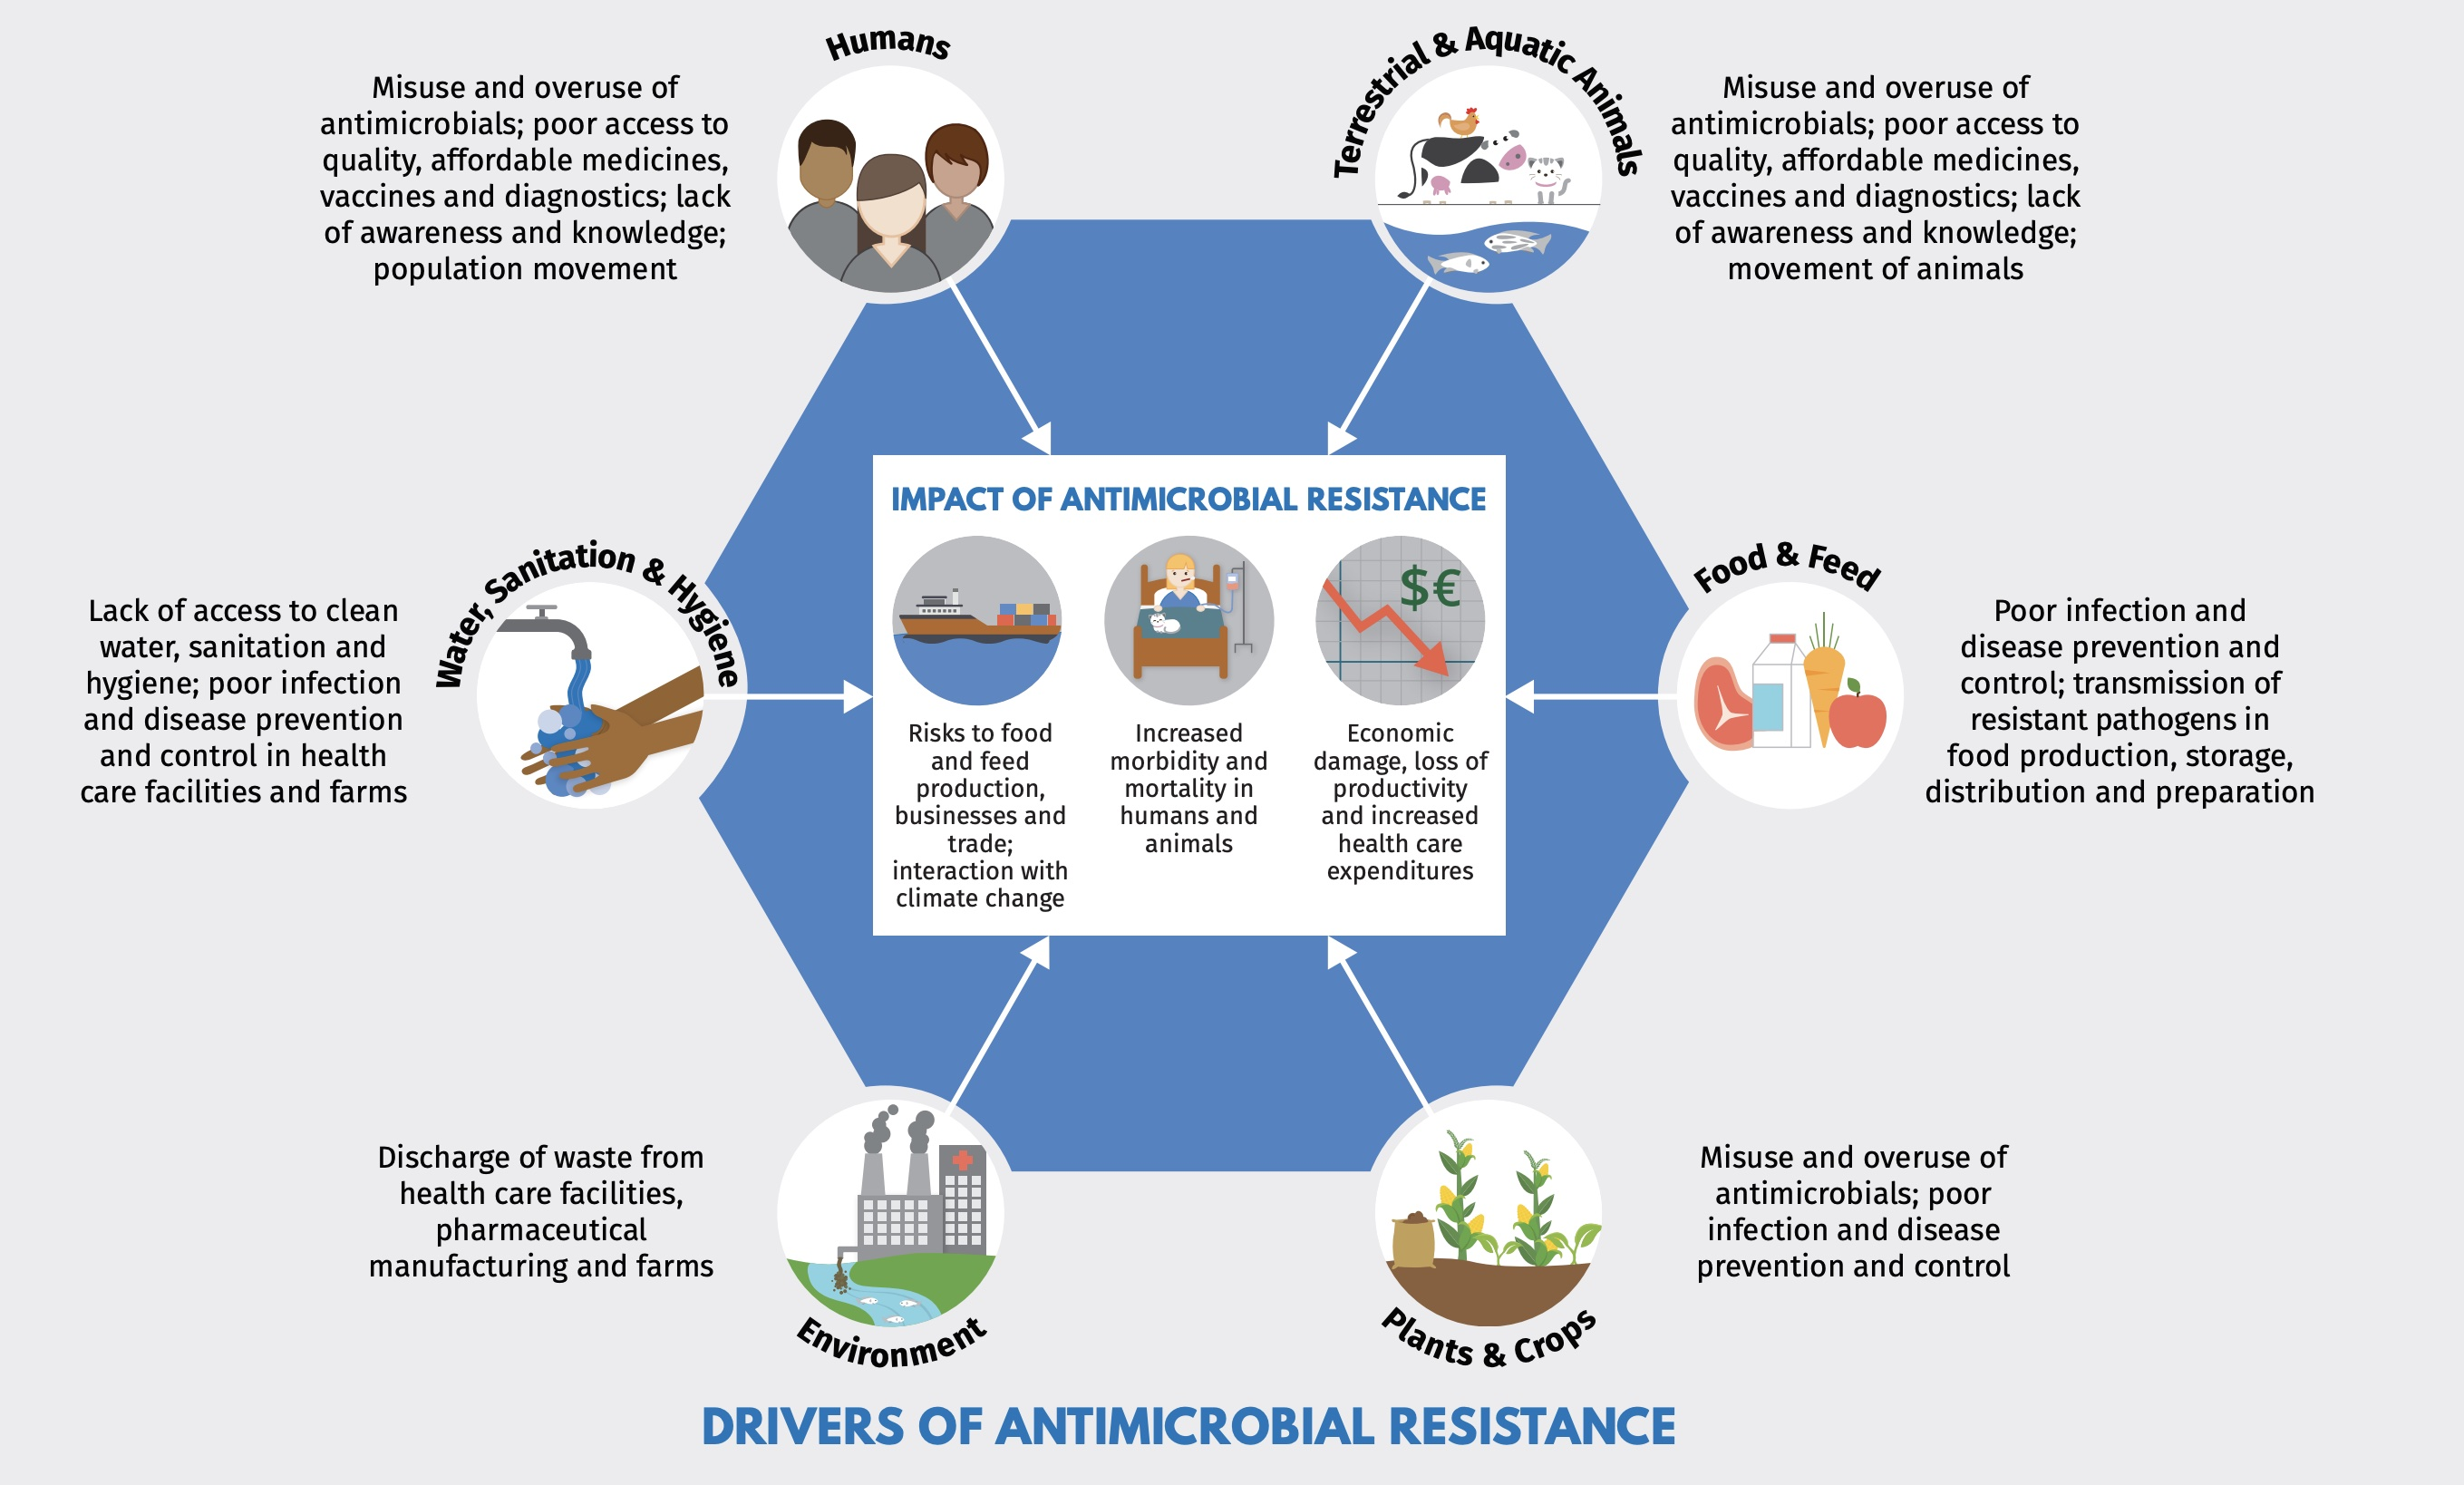
\includegraphics[width=8.33333in,height=\textheight]{images/onehealth.jpg}

Figure 6. Rationale for one-health model for addressing AMR: Source: WHO

\hypertarget{antibiotic-use-in-food-production}{%
\subsubsection*{Antibiotic use in food
production}\label{antibiotic-use-in-food-production}}
\addcontentsline{toc}{subsubsection}{Antibiotic use in food production}

\begin{itemize}
\tightlist
\item
  75\% if human infectious diseases that have emerged or re-emerged in
  recent decades are zoonotic-i.e.~they originated in animals (Woolhouse
  and Gowtage-Sequeria 2005).
\item
  Few antimicrobial classes are reserved exclusively for humans. The
  vast majority of antibiotics are used both in humans and animals,
  including domestic mammals, birds, farmed fish and shellfish,
  honeybees and others.
\item
  In horticulture, tetracyclines, streptomycin, and other antimicrobials
  are used for the prophylaxis and treatment of bacterial infections
  (e.g., fire blight \emph{Erwinea amylovora})
\item
  In veterinary medicine, there are major differences in the way
  antibiotics are used for companion animals (e.g., dogs, cats, pet
  birds, horses) versus food-producing animals. Antibiotic use in
  companion animals is broadly similar to humans to treat clinical
  infections or in select cases prophylaxis, such as post-surgery. In
  the case of food animals, if some animals are infected antibiotics may
  be administered through feed or water to the entire group for reasons
  of practicality or efficiency. \emph{Metaphylaxis is a term used to
  describe therapeutic/prophylaxis antibiotic treatment at a group
  level.}
\item
  The most controversial type of group treatment in food animals is
  long-term, low-dose mass antibiotic treatment for purposes of growth
  promotion. This practice has a high propensity to select for
  antimicrobial resistance and is driven by economic factors rather than
  treatment of clinical infection. The practice was banned by the EU in
  2006 but still continues in some countries such as the United States
  and China.
\item
  The reported benefits of using antibiotics for growth promotion is
  controversial ranges widely in the literature (1-10\%). Concerns have
  been expressed that antimicrobial growth promoters are often used to
  compensate for poor hygiene/housing and healthy management(McEwen and
  Collignon 2018).
\item
  Historically, governmental regulations have focused on toxicological
  dose-response data and the presence of antimicrobial residues in
  animal tissue, milk or other edible products (i.e.~eggs) from treated
  animals - \emph{so called minimum residue levels (MRLs) compatible
  with acceptable risk in humans.} While MRLs are well-understood and
  enforced withtesting programs and penalties, these programs do not
  take into account selection of antimicrobial-resistant pathogens.
\item
  The WHO has advocated for the termination of using antimicrobials for
  growth promotion. A recent
  \href{https://www.ecdc.europa.eu/sites/default/files/documents/JIACRA-III-Antimicrobial-Consumption-and-Resistance-in-Bacteria-from-Humans-and-Animals.pdf}{report
  from the ECDC} has suggested some progress in addressing this problem.
  Using surveillance data from 2017, the EU/EEA population mean
  antibiotic consumption in the 29 countries was 130 mg per kg of
  estimated biomass in humans and 108.3 mg per kg in food-producing
  animals (Fig 1.6). \emph{This first time since the agencies began
  publishing the joint reports in 2011 that antibiotic use in humans has
  exceeded use in livestock.} Consumption of third- and
  fourth-generation cephalosporins, fluoroquinolones, and
  aminopenicillins was considerably higher in human medicine, while
  consumption of macrolides was similar, and consumption of
  tetracyclines and polymyxins---a last-resort class of antibiotics that
  includes colistin---was significantly higher in food-producing
  animals.
\item
  In 2022, new
  \href{https://eur-lex.europa.eu/legal-content/EN/TXT/PDF/?uri=CELEX:32019R0006\&from=EN}{EU
  legislation} will prohibit all forms of routine antibiotic use in
  farming, including preventative group treatments and medicated feeding
  except in extraordinary circumstances.
\end{itemize}

Figure 7. Antibiotic use in livestock reported in 2010

\hypertarget{impacts-animal-antibiotic-use-on-human-amr}{%
\subsubsection*{Impacts Animal antibiotic use on Human
AMR}\label{impacts-animal-antibiotic-use-on-human-amr}}
\addcontentsline{toc}{subsubsection}{Impacts Animal antibiotic use on
Human AMR}

\hypertarget{case-study-cephalosporins}{%
\paragraph*{Case study-cephalosporins}\label{case-study-cephalosporins}}
\addcontentsline{toc}{paragraph}{Case study-cephalosporins}

Third generation cephalosporins (ceftotaxime, ceftriaxone) are widely
used for serious infections in humans, including the treatment of
urinary tract, abdominal, lung and bloodstream infections. These
antibiotics are classified as ``critically-important'' for human health
(\href{http://www.agisar.org/}{WHO AGISAR}). Cetiofur, cefpodoxime, and
cefoperazone are similar cephalosporins approved veterinary antibiotics
and used predominantly for treating bacterial infections in
food-producing animals including chickens and cattle.

Resistance to 3rd generation cephalosporins is mediated by
extended-spectrum beta-lactamases (ESBLs) and AmpC enzymes. ESBL genes
are highly mobile and transmitted on plasmids, transposons and other
genetic elements that can spread horizontally (to surrounding bacteria
and different bacterial species) and vertically (to daughter cells
through replication). Consequently, resistance can spread rapidly from
patient-to-patient and among different bacterial species. In recent
years, growing resistance to 3rd generation cephalosporins is common
among \emph{Escherichia coli} and \emph{Klebsiella pneumonia} has
required greater reliance on the few remaining classes of antimicrobials
such as carbapenems.

A number of studies comparing isolates from animals, food and human
infections have found a high genetic similarity or clonal isolates that
carry the same ESBL genes and plasmids colonizing animals used for food
production and isolates causing clinical infections in patients (Lazarus
et al. 2015).

Ceftiofur is frequently injected in small quantities to hatching eggs or
chicks as metaphylaxis for \emph{Escherichia coli} infections and/or
yolk sac infections (McEwen and Collignon 2018) (Fig1.7). This practice
has been shown to select for cephalosporin resistance in
\emph{Salmonella enterica} serovar Heidelberg- an important cause of
human illness in many countries that is typically associated with
consumption of contaminated poultry products (Smith et al. 2008).

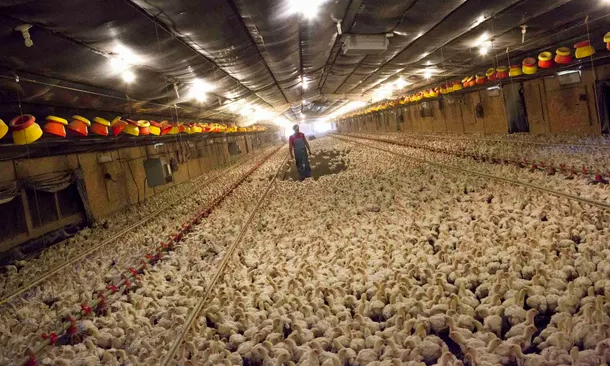
\includegraphics[width=5.20833in,height=\textheight]{images/chicken_farm.png}

Figure 8. Chicken farm in the United States of America.

Studies conducted by the Canadian Integrated Program for Antimicrobial
Resistance Surveillance detected a high degree of temporal correlation
in trends of resistance to ceftiofur and ceftriaxone (a drug of choice
for the treatment of severe cases of salmonellosis in children and
pregnant women) among \emph{Salmonella} Heidelberg from clinical
infections in humans, from poultry samples collected at retail stores,
and in \emph{E. coli} from poultry samples collected at retail
stores(Canada 2009). Voluntary termination of ceftiofur metaphylaxis in
hatcheries in the province of Quebec was followed by a precipitous drop
in the prevalence of resistance to ceftiofur; subsequent reintroduction
of ceftiofur in a more limited way was followed by a return to higher
levels of resistance (Fig 1.9)

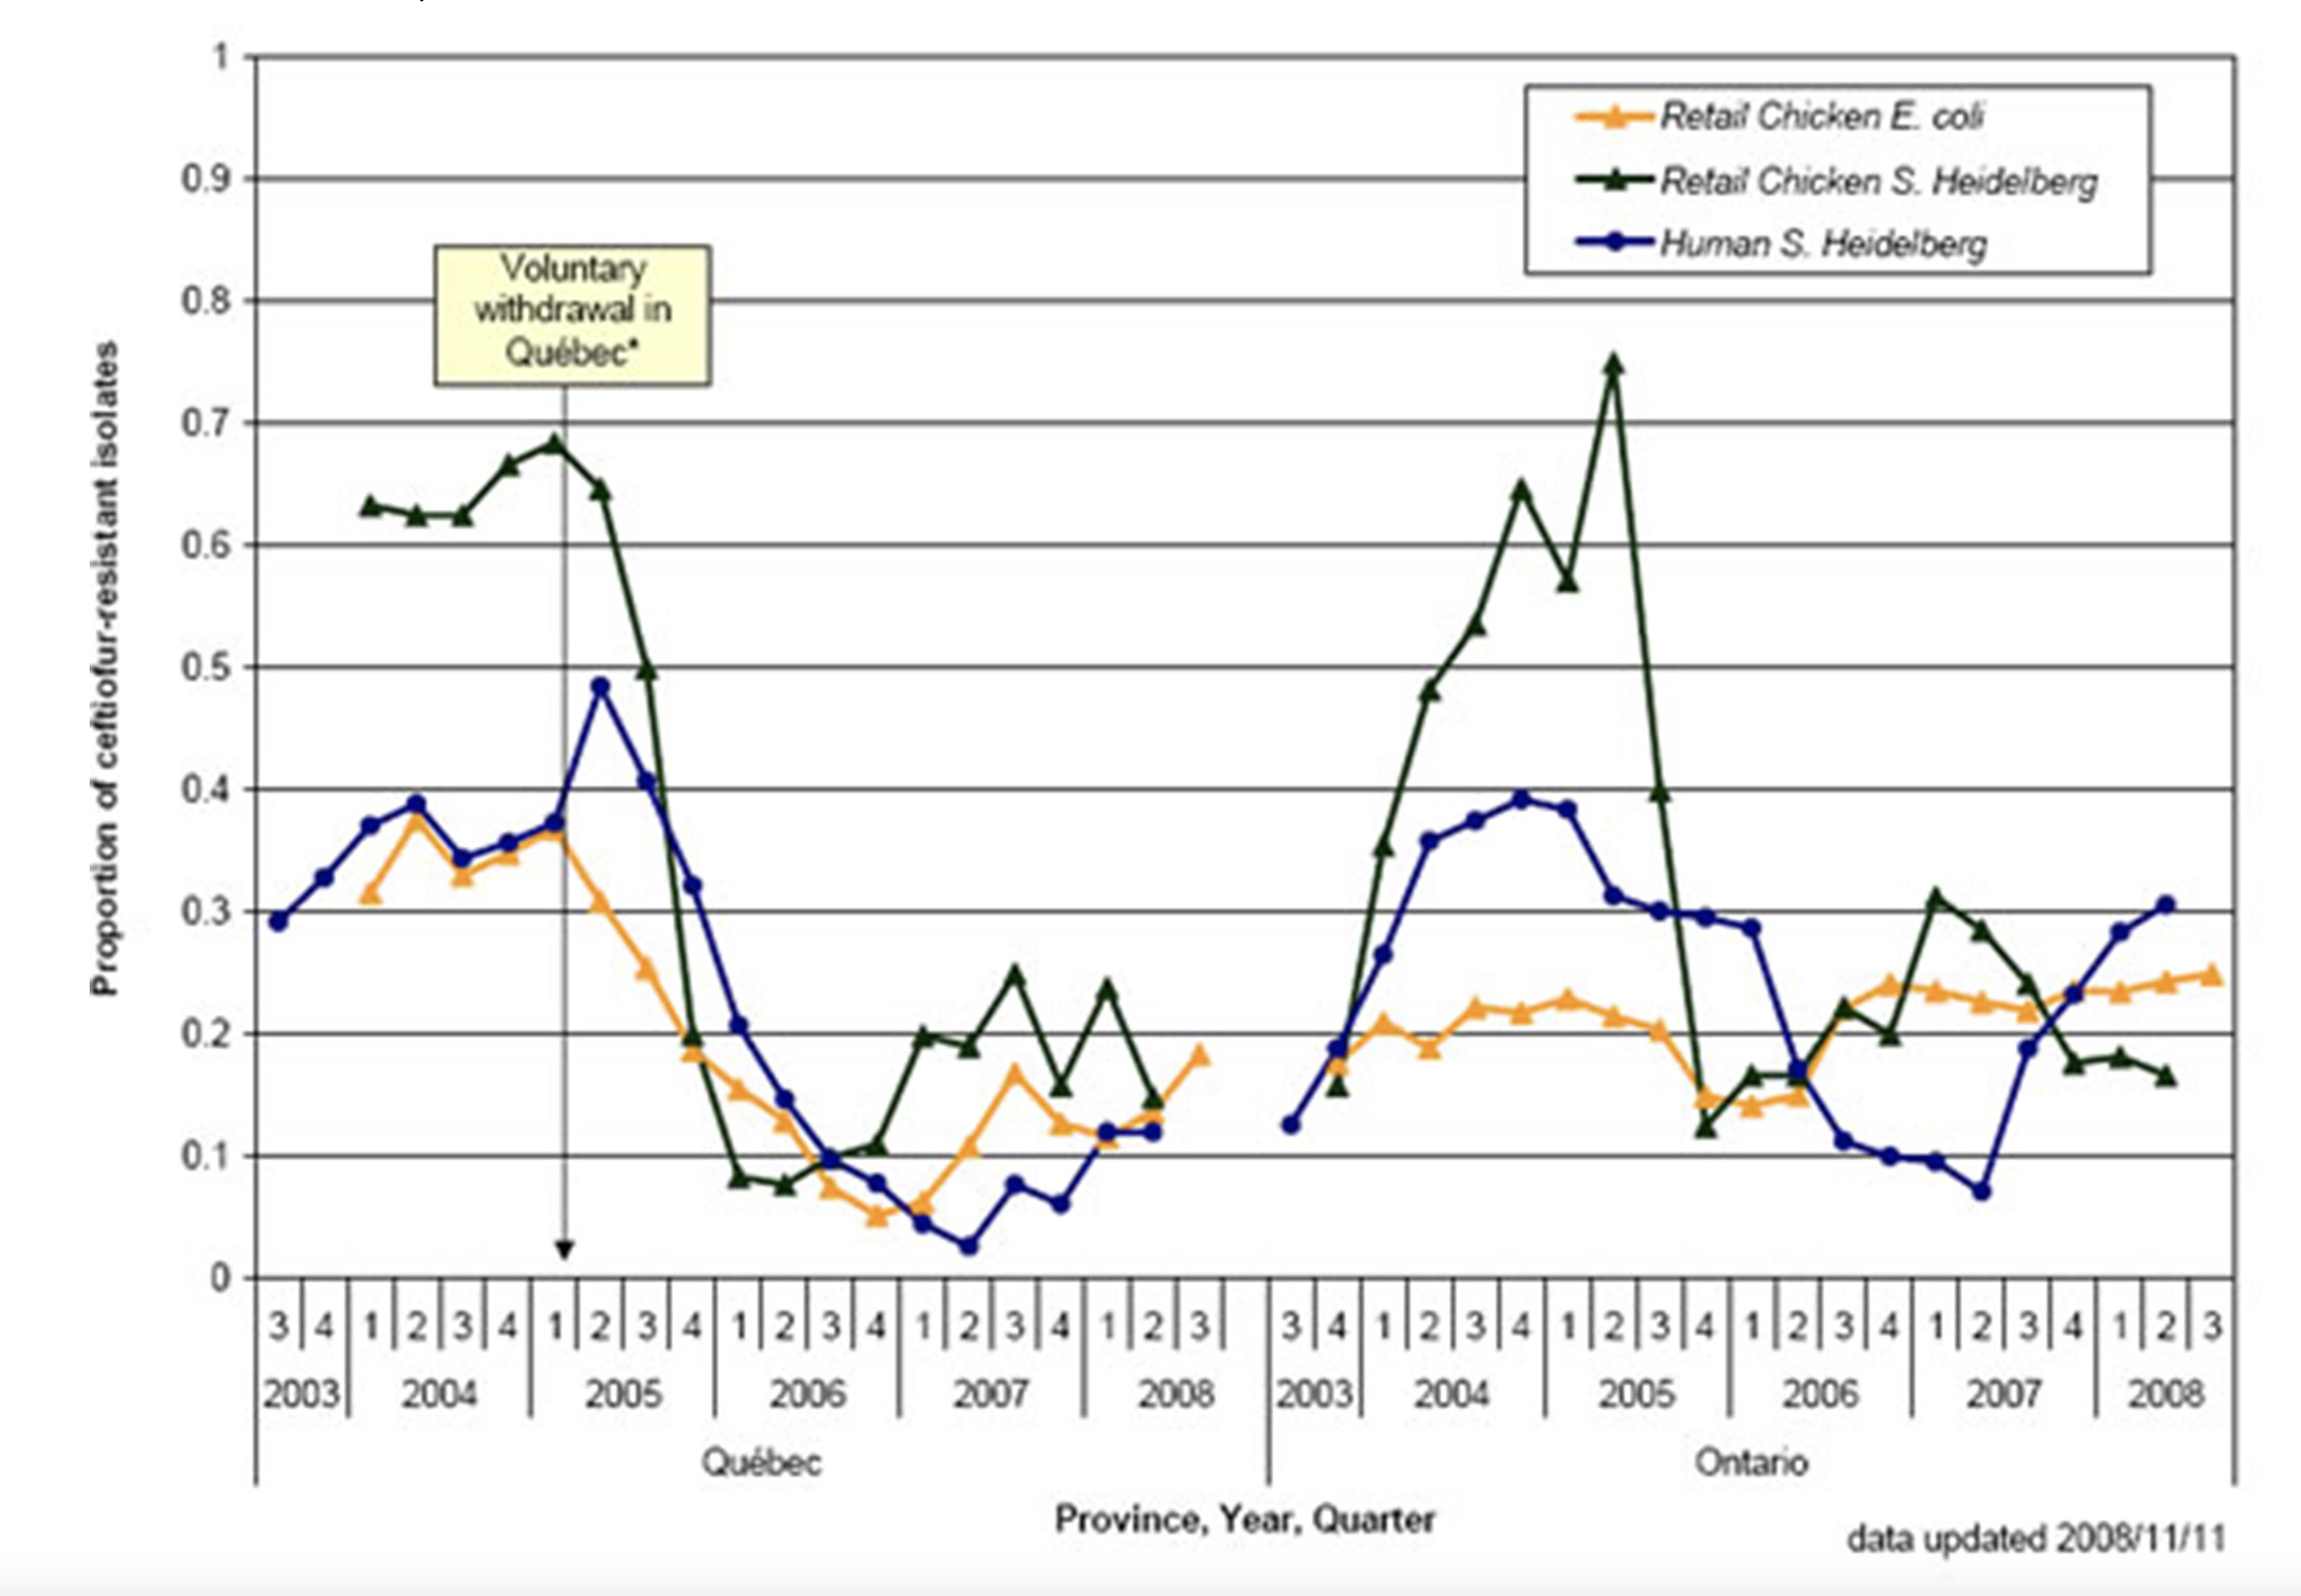
\includegraphics[width=5.20833in,height=\textheight]{images/Canada_ecoli.png}

Figure 9. Ceftiofur resistance in chicken and human \emph{Salmonella}
Heidelberg and chicken \emph{E. coli}.

In Japan, voluntary withdrawal of the off-label use of ceftiofur in
hatcheries in 2012 was also associated with significant decrease in
broad-spectrum cephalosporin resistance in \emph{E. coli} from chickens
prepared for cooking. Some other countries (e.g., Denmark) have placed
voluntary restrictions on its use. The label claim for day-old injection
of poultry flocks was withdrawn in Europe, while some countries have
banned off-label use of third-generation cephalosporins, and in other
countries there is a requirement that use be restricted to situations
where no other effective approved drugs are available for treatment.

These examples illustrate the danger of using antibiotics from the same
class as critical therapies used to treat human infections for
metaphylaxis or treatment in large numbers of animals. A similar pattern
in poultry was also observed with mass medication of poultry flocks
using fluoroquinolones antibiotics and selection of fluoroquinolone-
resistant \emph{Campylobacter jejuni} infections in humans (Endtz et al.
1991).

\hypertarget{case-study--colistin}{%
\paragraph*{Case study- colistin}\label{case-study--colistin}}
\addcontentsline{toc}{paragraph}{Case study- colistin}

Colistin is a member of the polymixin class of antibiotics, which have
been used in both human and veterinary medicine for over 50 years. Until
relatively recently, polymixins were rarely prescribed beyond topical or
inhalational therapy in rare cases because of dose-limiting
neurotoxicity and nephrotoxicity of the drugs.

However, use of intravenous colistin has surged in the last decade with
the increase in carbapenem-resistant \emph{Pseudomonas aeruginosa},
\emph{Acinetobacter baumannii} and \emph{Klebsiella pneumoniae.} Even as
human use has increased, colistin continues to be used in Brazil, Europe
and China a a growth promoting and antibiotic treatment for pigs,
poultry and calves.

\begin{itemize}
\item
  In 2014, colistin use in EU member states in animals was higher than
  humans with a reported 485 tonnes- 99.7\% in oral form or oral
  medicated feed (Agency 2016). In China, with the world's largest
  production of pigs and poultry, an estimated 12,000 tonnes of colistin
  was used in the food production industry (Liu et al. 2016).
\item
  In 2015, Lui and colleagues reported plasmid-mediated
  colistin-resistance gene, \emph{mcr-1}, in \emph{Escherichia coli}
  isolates obtained from animals, food and human bloodstream infections
  in China (Liu et al. 2016). Alarmingly, the resistance gene has also
  been detected in 5\% of healthy travellers from China in other parts
  of the world ({``Antibiotic Resistance\textemdash the Need for Global
  Solutions - {ScienceDirect},''} n.d.).
\item
  The \emph{mcr-1} gene has also been detected in isolates obtained from
  wildlife and surface water samples, demonstrating environmental
  contamination(Zurfuh et al., n.d.)
\item
  Additional plasmid-mediated colistin-resistance genes have been
  reported in many other bacterial species and countries, including
  \emph{mcr-2} from pigs in Belgium, and \emph{mcr-3,4,5} in other
  coutries(Borowiak et al. 2017)
\item
  Colistin illustrates important \emph{One-Health Dimensions} of AMR
  that differ from third generation cephaloporins. Specifically, large
  volumes of colistin use in animals, rather than humans, have probably
  have driven colistin resistance now observed in humans. Using large
  quantities of colistin for group treatment or growth promotion in
  animals has probably lead to antimicrobial resistance problems in
  human health, even through colistin was considered in the past to be
  less important because other less toxic treatments were still
  available.
\end{itemize}

\textbf{For further study:} In the 1990s avoparcin, a glycopeptide
antimicrobial, was widely used in growth promotion in pigs and poultry
production that was not initially thought to be of public health
importance. Surveillance and research were eventually able to show that
avoparcin use in animals contributed to the selection and wide
dissemination of what type of resistance?

\hypertarget{environmental-concerns}{%
\subsubsection*{Environmental concerns}\label{environmental-concerns}}
\addcontentsline{toc}{subsubsection}{Environmental concerns}

One health considers possible environmental drivers of AMR in additional
to human and animal health (McEwen and Collignon 2018). Many resistance
mechanisms such as beta-lactamases are millions of years old and
pre-date antibiotics. Soil and other environmental sources are rich
sources of highly-diverse populations of bacteria and genes.

Antimicrobial resistance to a wide variety of drugs has been
demonstrated in environmental bacteria isolated from the pre-antibiotic
era, as well as from various sites (e.g., caves) free of other sources
of exposure to modern antimicrobials. Yet their is abundant evidence
that human has an impact on the \emph{resistome}- the totality of or
resistance genes in the total environment (O'Neil 2015).

Hundreds of thousands of tonnes of antimicrobials are produced annually
and find their way into the environment. Waste from treatment plants and
the pharmaceutical industry especially if inadequately treated, has been
show to release high concentrations of antimicrobials into surface
water. Residues and metabolites of antimicrobials are constituents of
human sewage, livestock manure, and aquaculture, along with fecal
bacteria and resistance genes. Sewage treatment and composting of manure
reduce concentrations of some but not all antimicrobials and
micro-organisms, which are introduced to soil upon land application of
human and animal bio-solids (Rahube et al. 2016).

In developed countries with good-quality sewage and drinking water
treatment, and where most people have little to no direct contact with
food-producing animals, transmission of bacteria and resistance genes
from agricultural sources is largely foodborne, either from direct
contamination of meat and poultry during slaughter and processing, or
indirectly from fruit and vegetables contaminated by manure or
irrigation water. In countries with poor sewage and water treatment,
drinking water is likely to be very important in the transmission of
resistant bacteria and/or genes from animals. Poor sanitation also
facilitates indirect person-person water-borne transmission of enteric
bacteria among residents as well as international travellers who return
home colonized with resistant bacteria acquired locally. Through these
and other means, including globalized trade in animals and food and
long-distance migratory patterns of wildlife, antimicrobial-resistant
bacteria are globally disseminated.

General measures to address antimicrobial resistance in the wider
environment include improved controls on pollution from industrial,
residential, and agricultural sources. Improved research as well as
environmental monitoring and risk assessment are also required to better
understand the role of the environment in the selection and spread of
antimicrobial resistance and to identify more specific measures to
address resistance in this sector (Fig 1.9).

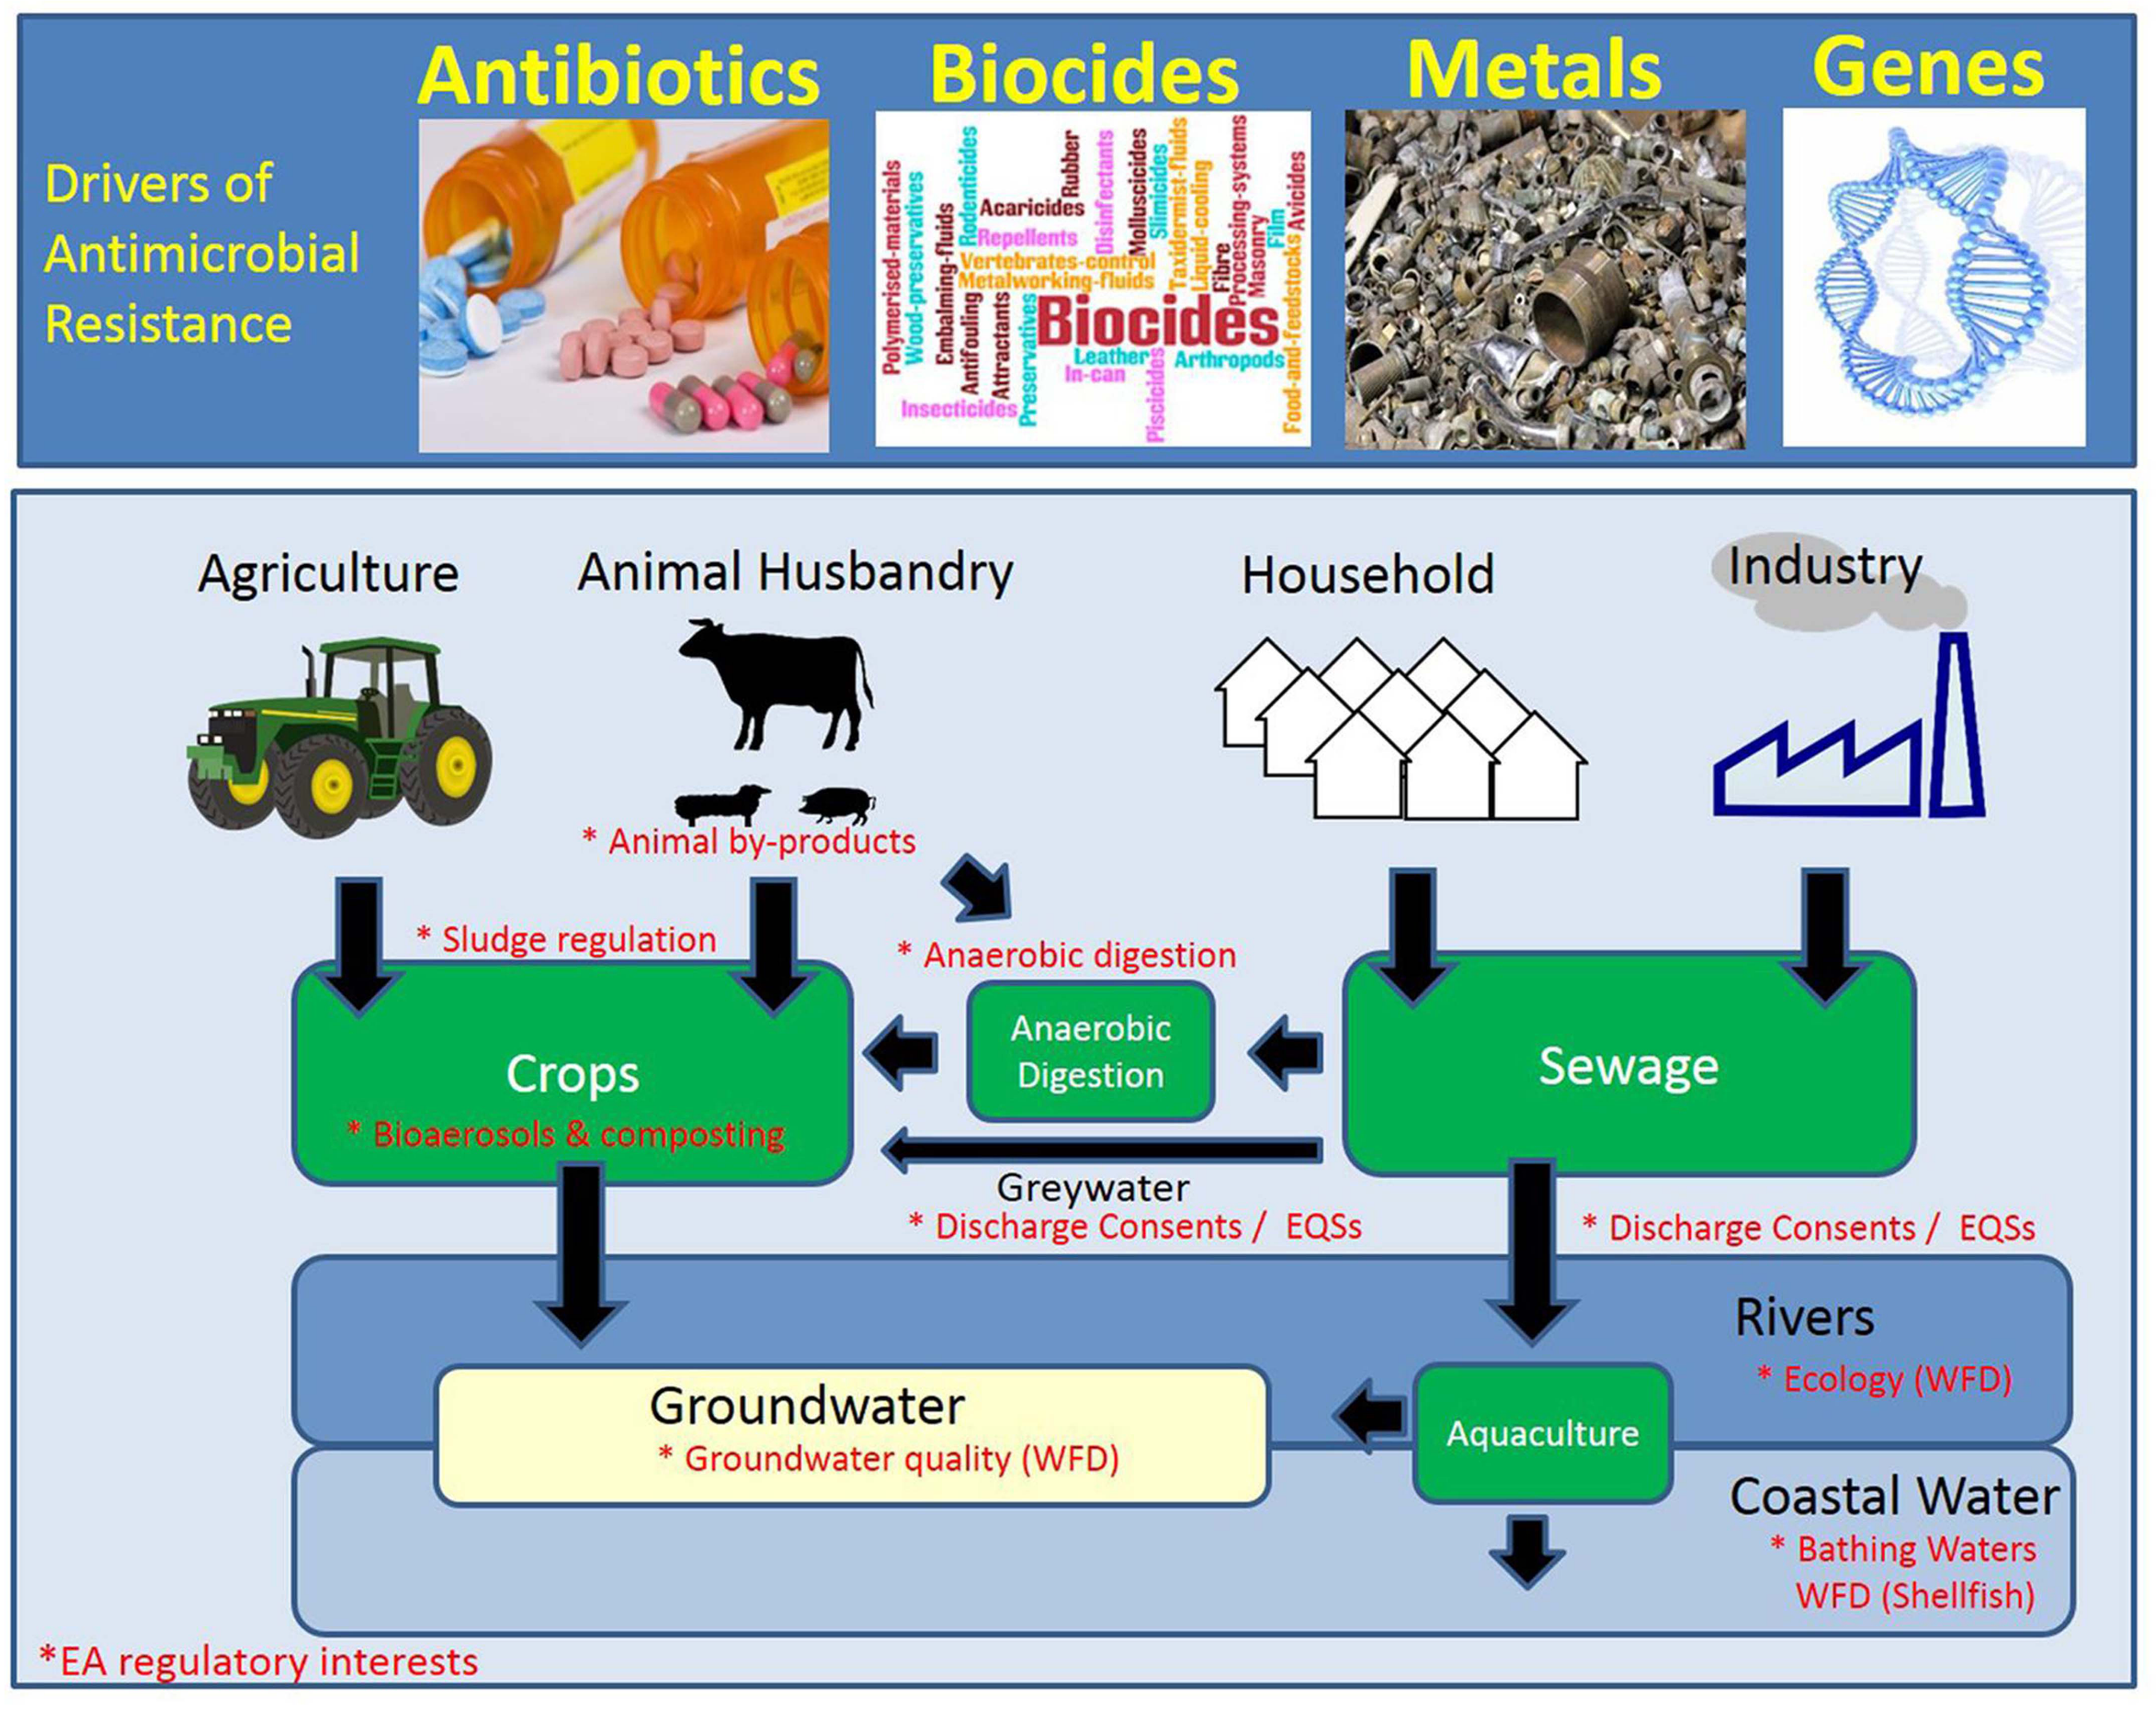
\includegraphics[width=5.20833in,height=\textheight]{images/hotspots.png}

Figure 10. Hotspots of antimicrobial resistance

\hypertarget{amr-in-low-middle-income-countries-lmics}{%
\subsection*{AMR in Low-Middle Income Countries
(LMICs)}\label{amr-in-low-middle-income-countries-lmics}}
\addcontentsline{toc}{subsection}{AMR in Low-Middle Income Countries
(LMICs)}

COVID-19 has focused global attention on the inequitable access to the
tools needed to control the pandemic, with high-income countries (HICs)
and low- and middle-income countries (LMICs) at opposite ends of the
scale. In the case of antibiotic resistance, a pandemic projected to
cause four times more deaths per year than occurred from COVID-19 during
2020, inequity between HICs and LMICs is a major challenge(Mendelson
2021):

\begin{itemize}
\tightlist
\item
  Lack of access to antibiotics in some poorer countries, a driver of
  mortality particularly in children under 5 years of age;
\item
  Lack of access to newer, expensive antibiotics needed to treat the
  increasing toll of MDR and XDR bacterial infections;
\item
  Inequity in ability to provide the basic public health interventions
  that drive many of the social determinants of infectious diseases in
  LMICs
\end{itemize}

The singular effectiveness of access to clean water, sanitation and
hygiene, called
\href{https://www.who.int/health-topics/water-sanitation-and-hygiene-wash}{WASH,}
in preventing the spread of disease is well understood, yet billions of
people around the world still lack access to these necessities (Bürgmann
et al. 2018).

\begin{itemize}
\tightlist
\item
  Currently, 2.1 billion people live without access to safe drinking
  water and 4.5 billion people are without access to adequate
  sanitation.
\item
  Every day, 1300 children under 5 die from preventable diarrhoeal
  diseases, including cholera, caused by contaminated water and poor
  sanitation.
\item
  1 in 3 healthcare facilities lacks soap and water or hand sanitizer
  where staff provide patient care. Billions of patients worldwide must
  rely on these facilities.
\item
  In some countries, up to 90\% of women receive routine prophylactic
  antibiotics during childbirth, highlighting the conditions under which
  they are delivering their babies and what would cause the
  inevitability of infection
\end{itemize}

The cumulative lack of WASH adds up to children and adults not only
getting unnecessarily sick---with the associated suffering, medical
costs and loss of income or schooling---they are relying on antibiotics
to get better (Denny 2021a). The challenge here is that WASH is a public
works solution for a public health problem. WASH is not a pill or `quick
fix'. It requires capital investment, system strengthening, and
behaviour change to ensure that clean water and functional toilets are
available and utilized day-in and day-out. These issues require a
different set of skills than those possessed by medical and public
health professionals.

In LMICs, an estimated 670 million people still practice
\href{https://blogs.worldbank.org/opendata/open-defeca\%20tion-nearly-halved-2000-still-practiced-670-million}{open
defaecation in 2017}, and only one in three people have access to safe
drinking water, resulting in high rates of diarrheal disease and equally
large amounts of inappropriate antibiotic use (Denny 2021b). According
to
\href{https://www.who.int/news-room/\%20fact-sheets/detail/immunization-coverage.}{WHO
surveys}, vaccination, a cornerstone of infection prevention and
reducing the need for antibiotic use, is suboptimal in both HICs and
LMICs. In 2019, global third-dose coverage for childhood pneumococcal
vaccination in 149 member states was only 48\%, and global rotavirus
vaccine coverage was estimated at 39\%. In South Africa, middle-income
country, procures less than 1 million doses of influenza vaccine for its
annual influenza season, despite in excess of 10 million people being
identified as high-risk for influenza and prioritized for vaccination
(Mendelson 2021).

Optimizing infection prevention on farms and making improvements to
housing conditions and feed to reduce illness in animals is also
critical in food production to offset the need for antibiotic growth
promotion or metaphylaxis in food production animals. While there has
been progress in the reduction of antibiotic use in farms in the EU and
other HICs, attention nor funding for such improvements in LMICs has not
even been proposed. ``It's one thing being told to reduce your
antibiotic use in food production, it's another to have the means to do
so, even for the most committed resource-poor farmer''(Mendelson 2021).

As discussed above, the emergence of antimicrobial resistance (AMR) is a
complex phenomenon and is intensified by selective pressure through
antibiotic use in humans, animals, and agriculture. The transmission of
AMR to humans occurs from contact with animals (including food), other
humans, and the environment. Transmission is facilitated by several
factors, including high population density, lack of access to clean
water, suboptimal sewage systems, poor sanitation, and poor healthcare
infection control practices, all of which are more common in LMICs. With
the increasing consumption of antimicrobials in humans, lack of
regulation on antimicrobial use in farming, and pharmaceutical industry
pollution, it may not be surprising that relatively higher levels of AMR
among human pathogens are being reported from LMIC (Fig 10).

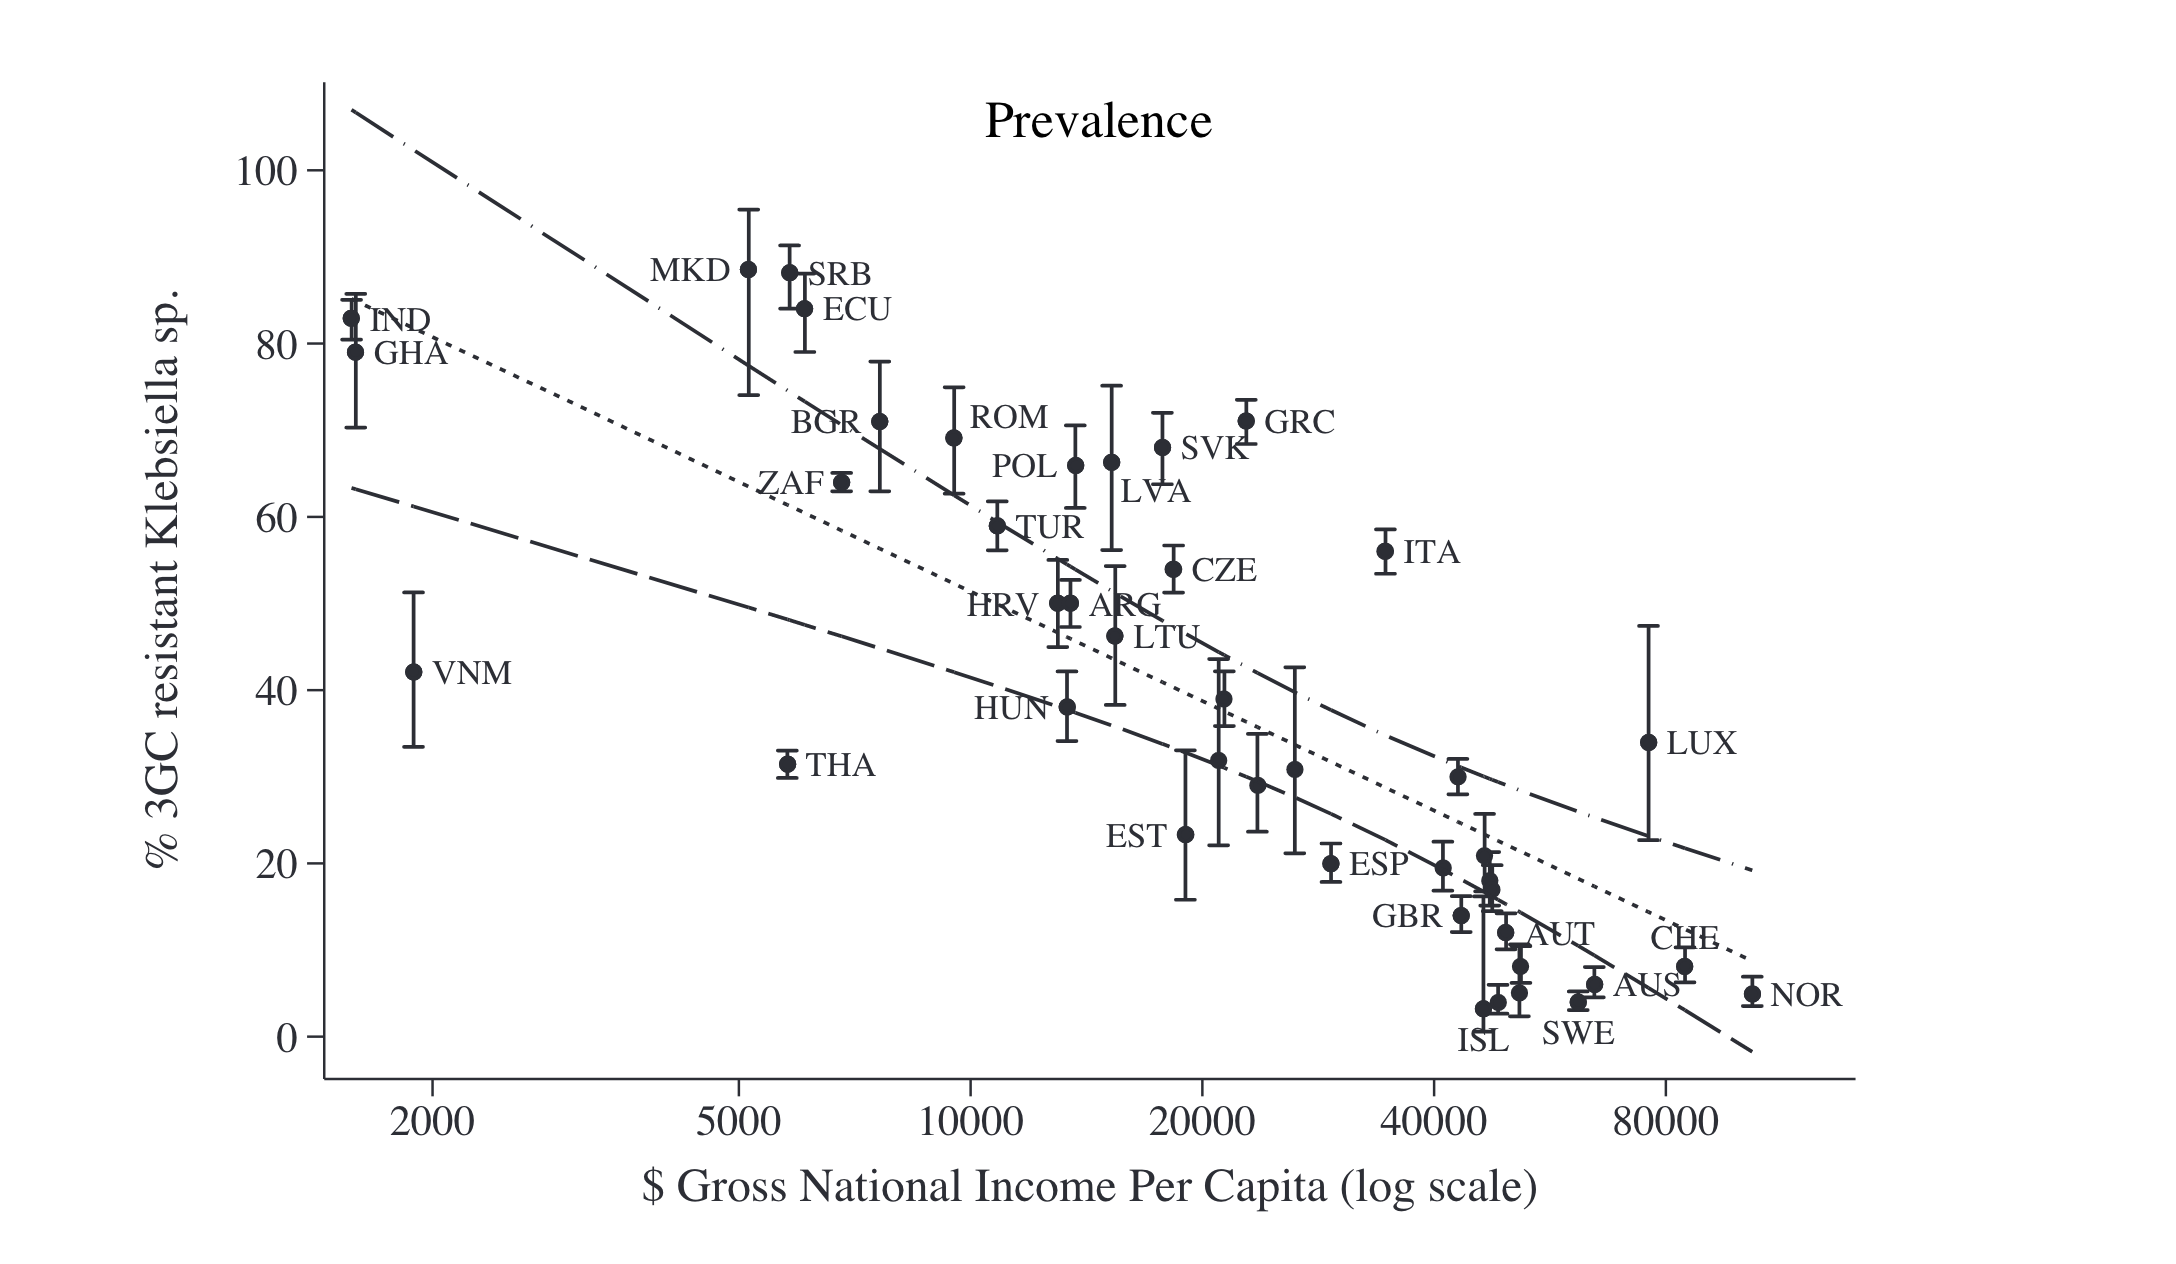
\includegraphics[width=6.25in,height=\textheight]{images/gdp.png}

Figure 10. Prevalence of third-generation cephalosporin-resistant
(3GCR)Klebsiella spp.by gross national income per capita and predicted
values with 95\% confidence intervals according to a linear regression
model. Data are from reference (Alvarez-Uria, Gandra, and Laxminarayan
2016).

The international focus on awareness, surveillance, infection
prevention, stewardship and research and development (R\&D) of new
antibiotics is actually widening the equity gap by pouring millions of
dollars into R\&D of new antibiotics and surveillance systems, while the
intervention that could benefit LMICs the most, infection prevention,
has received a relatively few resources.

What are the possible solutions? Recently COVID-19 has refocused
attention that in infectious diseases The Access to COVID-19 Tools
(ACT)-Accelerator that we will discuss in Model 2 has shown that
financial contributions from HICs to a LMIC-pool can improve equitable
access to diagnostics, therapeutics and vaccines, but it is conceivable
that the same model could be broadened to encompass tools that would
support major social change for AMR.

\hypertarget{cross-border-spread-of-amr}{%
\subsection*{Cross-border spread of
AMR}\label{cross-border-spread-of-amr}}
\addcontentsline{toc}{subsection}{Cross-border spread of AMR}

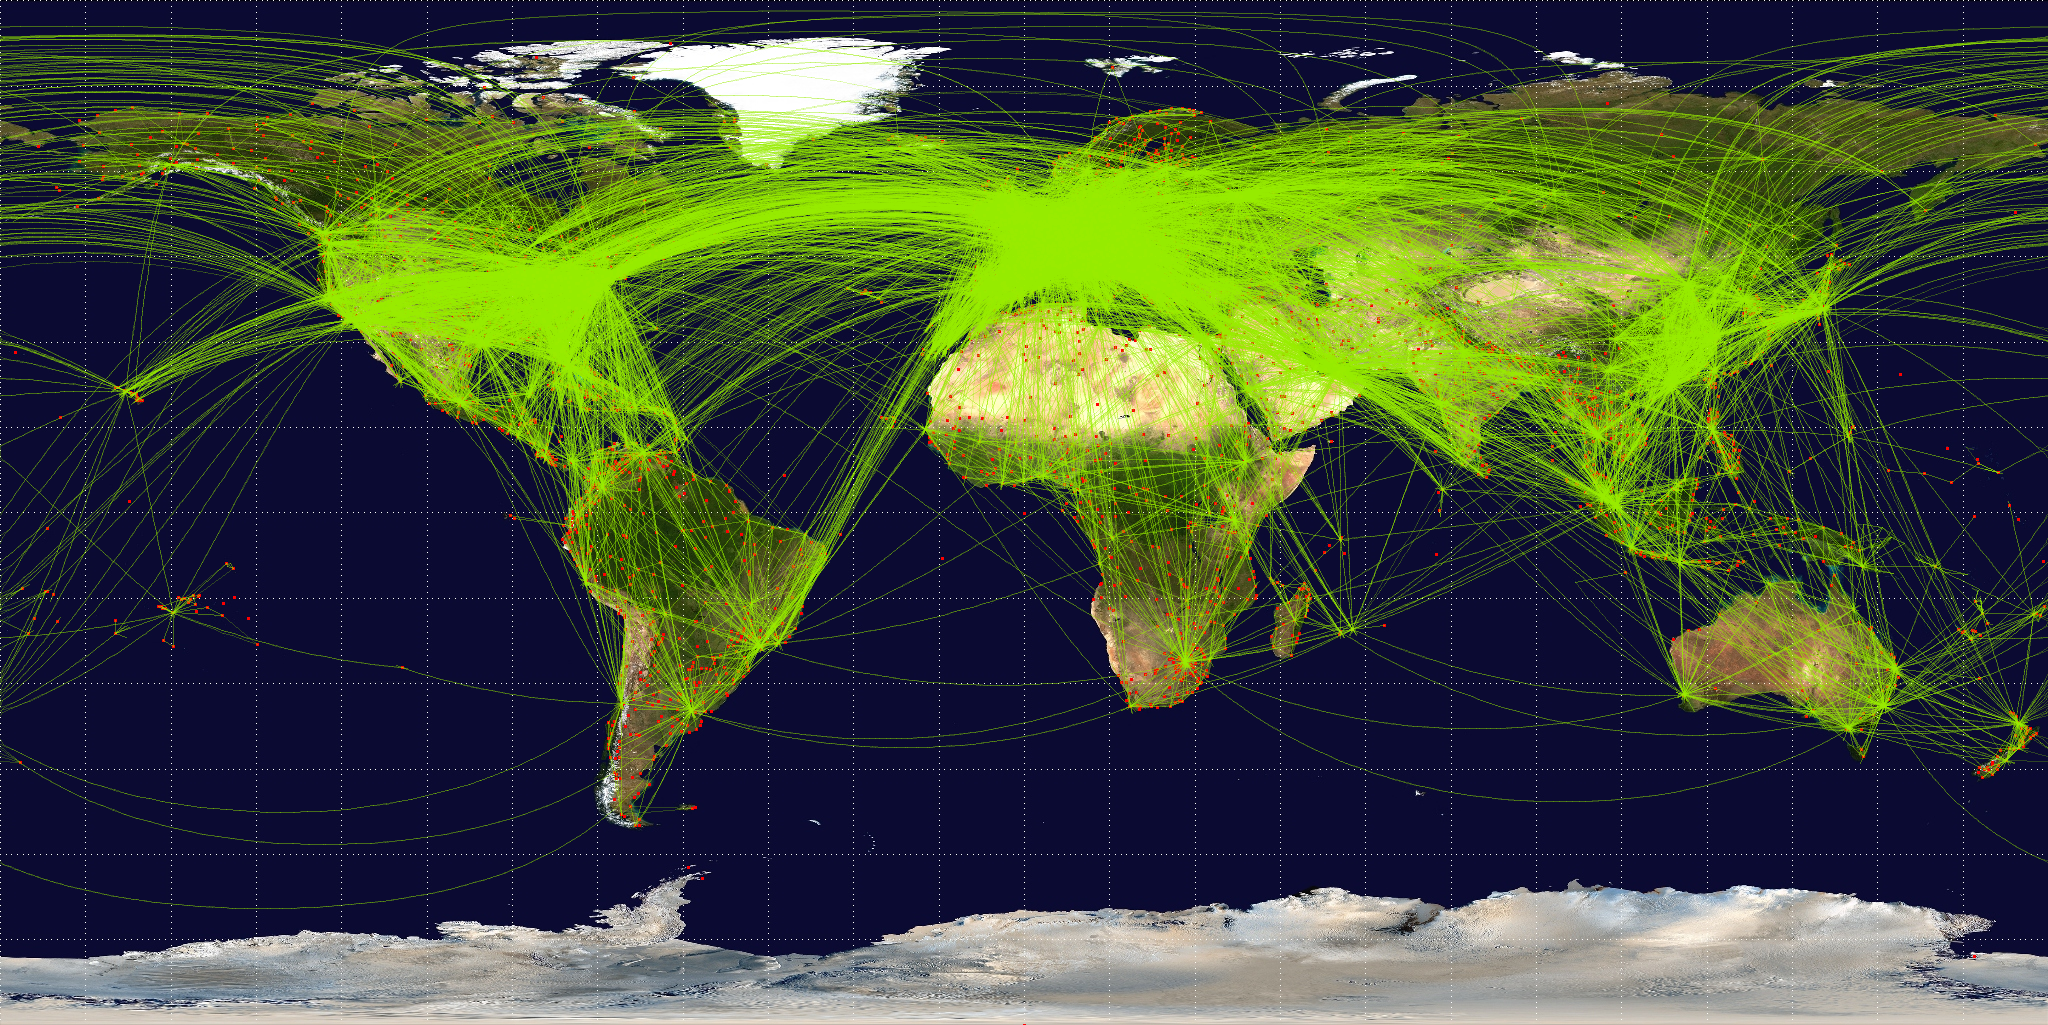
\includegraphics[width=5.20833in,height=\textheight]{images/worldairlineroute2014.png}

Figure 11. World airline travel routes in 2014

The COVID-19 pandemic has exposed the limitations of global
collaboration and response within existing global health frameworks,
pointing to a clear need for more rules-based global governance to be
able to effectively prevent, prepare and respond to health emergencies
in a more just equitable way. However, valuable lessons from COVID-19
pandemic could enhance actions against AMR. (Table 1.2). Clearly,
actions taken by one country have had substantial consequences for
others. governments should significantly bolster global and national
capacity to prevent and respond to global cross-border health threats
more broadly.

Table 1.2 Global successes and shortcomings in the multilateral response
to the COVID-19 pandemic. Table is from Jit et al 2021 (Jit et al.
2021).

\begin{longtable}[]{@{}
  >{\raggedright\arraybackslash}p{(\columnwidth - 4\tabcolsep) * \real{0.1688}}
  >{\raggedright\arraybackslash}p{(\columnwidth - 4\tabcolsep) * \real{0.4586}}
  >{\raggedright\arraybackslash}p{(\columnwidth - 4\tabcolsep) * \real{0.3726}}@{}}
\toprule
\begin{minipage}[b]{\linewidth}\raggedright
Domain
\end{minipage} & \begin{minipage}[b]{\linewidth}\raggedright
Successes
\end{minipage} & \begin{minipage}[b]{\linewidth}\raggedright
Shortcomings
\end{minipage} \\
\midrule
\endhead
\textbf{Research collaboration and information sharing} &
\begin{minipage}[t]{\linewidth}\raggedright
\begin{itemize}
\item
  Sharing of information by researchers
\item
  International research collaborations
\item
  Public data repositories
\end{itemize}
\end{minipage} & \begin{minipage}[t]{\linewidth}\raggedright
\begin{itemize}
\item
  Many regions and countries slow to learn policy lessons from elsewhere
\item
  Lack of systemic global research governance
\item
  Duplication of research studies
\end{itemize}
\end{minipage} \\
\textbf{Vaccine discovery and development} &
\begin{minipage}[t]{\linewidth}\raggedright
\begin{itemize}
\item
  Multinational initiatives to fund efforts such as the Coronavirus
  Global Response and the Coalition for Epidemic Preparedness
  Innovations
\item
  Approval of vaccines and adjuvants
\item
  Establishing the principle of equitable vaccine distribution through
  the COVAX Facility (despite failures in implementation)
\end{itemize}
\end{minipage} & \begin{minipage}[t]{\linewidth}\raggedright
\begin{itemize}
\item
  Most funding from national efforts
\item
  Most vaccine doses secured by rich countries through bilateral deals
\item
  Trade barriers around vaccines and raw materials
\end{itemize}
\end{minipage} \\
\textbf{Travel policies} & \begin{minipage}[t]{\linewidth}\raggedright
\begin{itemize}
\tightlist
\item
  Travel restrictions delayed spread from China in early 2020
\end{itemize}
\end{minipage} & \begin{minipage}[t]{\linewidth}\raggedright
\begin{itemize}
\item
  Dissonant COVID-19 response policies between highly connected nations
\item
  Restrictions on travel to countries of high COVID-19 incidence
  contribute little to control in these countries
\end{itemize}
\end{minipage} \\
\bottomrule
\end{longtable}

The actions of the EU during the pandemic illustrate the tension between
short-term nationalistic incentives and long-term imperatives for
cooperation towards achieving global public goods such as reducing
antimicrobial resistance. The EU has struggled to balance preferences of
individual member-states (and those of their political leaderships),
with the collective interests of all member-states. Such tensions are
especially challenging when health care and health policy issues are
involved, given how these have hitherto remained largely the
responsibility of the member-states. In a pandemic, this can lead to
inertia and political indecisiveness at the EU level, with member-states
filling the gap with potentially contradictory or competing decisions.

Looking ahead, it is likely that there will be several changes to the
global health architecture, possibly including a new pandemic treaty and
additional international collaborative mechanisms to promote
preparedness and coordinate responses. In the following sections, we
explore what those developments might look like in three key areas.

\hypertarget{summary}{%
\subsection*{Summary}\label{summary}}
\addcontentsline{toc}{subsection}{Summary}

The post-COVID-19 world must overcome the serious setbacks from the
pandemic to hard-fought progress in reducing poverty and inequality.
Health infrastructure and human resources vital for fighting AMR have
been overburdened and will take many years to recover, particularly if
governments impose austerity measures as they seek to recover from
fiscal expansion during the pandemic.

Decades of funding neglect, combined with continuously increasing global
antibiotic consumption, poor surveillance data, and weak pipelines for
new drugs, vaccines and diagnostics, has left the world dangerously
vulnerable to a pandemic of resistant and untreatable infections.

Therefore, strong multilateral collaboration is essential for the world
to absorb these shocks and refocus on the silent but growing pandemic of
AMR. Pandemics are opportunities to re-imagine governance structures and
learn from previous experiences. COVID-19 has shown the importance of
multilateral collaboration in diverse areas, including research and
knowledge sharing, discovery, development and distribution of vaccines
and medicines and access to diagnostics and medicines. Action is needed
now to reverse the unthinkable future of untreatable infections.

\hypertarget{lecture-slides}{%
\subsection*{Lecture Slides}\label{lecture-slides}}
\addcontentsline{toc}{subsection}{Lecture Slides}

\hypertarget{references}{%
\subsection*{References}\label{references}}
\addcontentsline{toc}{subsection}{References}

\hypertarget{refs}{}
\begin{CSLReferences}{1}{0}
\leavevmode\vadjust pre{\hypertarget{ref-EuropeanMedicinesAgency2016}{}}%
Agency, European Medicines. 2016. \emph{Updated Advice on the Use of
Colistin Products in Animals Within the {European Union}: Development of
Resistance and Possible Impact on Human and Animal Health}.

\leavevmode\vadjust pre{\hypertarget{ref-Alvarez-UriaEtAl2016}{}}%
Alvarez-Uria, Gerardo, Sumanth Gandra, and Ramanan Laxminarayan. 2016.
{``Poverty and Prevalence of Antimicrobial Resistance in Invasive
Isolates.''} \emph{International Journal of Infectious Diseases} 52
(November): 59--61. \url{https://doi.org/10.1016/j.ijid.2016.09.026}.

\leavevmode\vadjust pre{\hypertarget{ref-zotero-7665}{}}%
{``Antibiotic Resistance\textemdash the Need for Global Solutions -
{ScienceDirect}.''} n.d.
https://www-sciencedirect-com.ezproxy.unibo.it/science/article/pii/S1473309913703189?via\%3Dihub.

\leavevmode\vadjust pre{\hypertarget{ref-BorowiakEtAl2017}{}}%
Borowiak, Maria, Jennie Fischer, Jens A. Hammerl, Rene S. Hendriksen,
Istvan Szabo, and Burkhard Malorny. 2017. {``Identification of a Novel
Transposon-Associated Phosphoethanolamine Transferase Gene, Mcr-5,
Conferring Colistin Resistance in d-Tartrate Fermenting {Salmonella}
Enterica Subsp. Enterica Serovar {Paratyphi B}.''} \emph{The Journal of
Antimicrobial Chemotherapy} 72 (12): 3317--24.
\url{https://doi.org/10.1093/jac/dkx327}.

\leavevmode\vadjust pre{\hypertarget{ref-BurgmannEtAl2018}{}}%
Bürgmann, Helmut, Dominic Frigon, William H Gaze, Célia M Manaia, Amy
Pruden, Andrew C. Singer, Barth F Smets, and Tong Zhang. 2018. {``Water
and Sanitation: An Essential Battlefront in the War on Antimicrobial
Resistance.''} \emph{FEMS Microbiology Ecology} 94 (9).
\url{https://doi.org/10.1093/femsec/fiy101}.

\leavevmode\vadjust pre{\hypertarget{ref-Canada2009}{}}%
Canada, Public Health Agency of. 2009. {``{ARCHIVED} - {UPDATE} -
{Salmonella Heidelberg Ceftiofur}-{Related Resistance} in {Human} and
{Retail Chicken Isolates} - 2006 to 2008.''} Datasets;Research.
https://www.canada.ca/en/public-health/services/surveillance/canadian-integrated-program-antimicrobial-resistance-surveillance-cipars/update-salmonella-heidelberg-ceftiofur-related-resistance-human-retail-chicken-isolates-2006-2008.html.

\leavevmode\vadjust pre{\hypertarget{ref-Denny2021}{}}%
Denny, Lindsay. 2021b. {``{BSAC Vanguard Series}: Clean
Water\textemdash the World's Best Medicine for Disease and
Drug-Resistant Infection.''} \emph{Journal of Antimicrobial
Chemotherapy}, no. dkab414 (November).
\url{https://doi.org/10.1093/jac/dkab414}.

\leavevmode\vadjust pre{\hypertarget{ref-Denny2021a}{}}%
---------. 2021a. {``{BSAC Vanguard Series}: Clean Water\textemdash the
World's Best Medicine for Disease and Drug-Resistant Infection.''}
\emph{Journal of Antimicrobial Chemotherapy}, no. dkab414 (November).
\url{https://doi.org/10.1093/jac/dkab414}.

\leavevmode\vadjust pre{\hypertarget{ref-EndtzEtAl1991}{}}%
Endtz, H. P., G. J. Ruijs, B. van Klingeren, W. H. Jansen, T. van der
Reyden, and R. P. Mouton. 1991. {``Quinolone Resistance in Campylobacter
Isolated from Man and Poultry Following the Introduction of
Fluoroquinolones in Veterinary Medicine.''} \emph{The Journal of
Antimicrobial Chemotherapy} 27 (2): 199--208.
\url{https://doi.org/10.1093/jac/27.2.199}.

\leavevmode\vadjust pre{\hypertarget{ref-HolmesEtAl2016b}{}}%
Holmes, Alison H, Luke S P Moore, Arnfinn Sundsfjord, Martin Steinbakk,
Sadie Regmi, Abhilasha Karkey, Philippe J Guerin, and Laura J V Piddock.
2016. {``Understanding the Mechanisms and Drivers of Antimicrobial
Resistance.''} \emph{The Lancet} 387 (10014): 176--87.
\url{https://doi.org/10.1016/S0140-6736(15)00473-0}.

\leavevmode\vadjust pre{\hypertarget{ref-JitEtAl2021}{}}%
Jit, Mark, Aparna Ananthakrishnan, Martin McKee, Olivier J. Wouters,
Philippe Beutels, and Yot Teerawattananon. 2021. {``Multi-Country
Collaboration in Responding to Global Infectious Disease Threats:
Lessons for {Europe} from the {COVID}-19 Pandemic.''} \emph{The Lancet
Regional Health \textendash{} Europe} 9 (October).
\url{https://doi.org/10.1016/j.lanepe.2021.100221}.

\leavevmode\vadjust pre{\hypertarget{ref-KadriEtAl2018a}{}}%
Kadri, Sameer S, Jennifer Adjemian, Yi Ling Lai, Alicen B Spaulding,
Emily Ricotta, D Rebecca Prevots, Tara N Palmore, et al. 2018.
{``Difficult-to-{Treat Resistance} in {Gram}-Negative {Bacteremia} at
173 {US Hospitals}: Retrospective {Cohort Analysis} of {Prevalence},
{Predictors}, and {Outcome} of {Resistance} to {All First}-Line
{Agents}.''} \emph{Clinical Infectious Diseases} 67 (12): 1803--14.
\url{https://doi.org/10.1093/cid/ciy378}.

\leavevmode\vadjust pre{\hypertarget{ref-LazarusEtAl2015}{}}%
Lazarus, Benjamin, David L. Paterson, Joanne L. Mollinger, and Benjamin
A. Rogers. 2015. {``Do Human Extraintestinal {Escherichia} Coli
Infections Resistant to Expanded-Spectrum Cephalosporins Originate from
Food-Producing Animals? A Systematic Review.''} \emph{Clinical
Infectious Diseases: An Official Publication of the Infectious Diseases
Society of America} 60 (3): 439--52.
\url{https://doi.org/10.1093/cid/ciu785}.

\leavevmode\vadjust pre{\hypertarget{ref-LiuEtAl2016a}{}}%
Liu, Yi-Yun, Yang Wang, Timothy R Walsh, Ling-Xian Yi, Rong Zhang, James
Spencer, Yohei Doi, et al. 2016. {``Emergence of Plasmid-Mediated
Colistin Resistance Mechanism {MCR}-1 in Animals and Human Beings in
{China}: A Microbiological and Molecular Biological Study.''} \emph{The
Lancet Infectious Diseases} 16 (2): 161--68.
\url{https://doi.org/10.1016/S1473-3099(15)00424-7}.

\leavevmode\vadjust pre{\hypertarget{ref-MagiorakosEtAl2012a}{}}%
Magiorakos, A. -P., A. Srinivasan, R. B. Carey, Y. Carmeli, M. E.
Falagas, C. G. Giske, S. Harbarth, et al. 2012. {``Multidrug-Resistant,
Extensively Drug-Resistant and Pandrug-Resistant Bacteria: An
International Expert Proposal for Interim Standard Definitions for
Acquired Resistance.''} \emph{Clinical Microbiology and Infection} 18
(3): 268--81. \url{https://doi.org/10.1111/j.1469-0691.2011.03570.x}.

\leavevmode\vadjust pre{\hypertarget{ref-McEwenCollignon2018}{}}%
McEwen, Scott A., and Peter J. Collignon. 2018. {``Antimicrobial
{Resistance}: A {One Health Perspective}.''} \emph{Microbiology
Spectrum} 6 (2): 6.2.10.
\url{https://doi.org/10.1128/microbiolspec.ARBA-0009-2017}.

\leavevmode\vadjust pre{\hypertarget{ref-Mendelson2021}{}}%
Mendelson, Marc. 2021. {``{BSAC Vanguard Series}: Inequality and
Antibiotic Resistance.''} \emph{Journal of Antimicrobial Chemotherapy},
no. dkab426 (November). \url{https://doi.org/10.1093/jac/dkab426}.

\leavevmode\vadjust pre{\hypertarget{ref-ONeilJim2015}{}}%
O'Neil, Jim. 2015. \emph{Antimicrobials in Agriculture and the
Environment: Reducing Unnecessary Use and Waste.{The} Review on
Antimicrobial Resistance.}

\leavevmode\vadjust pre{\hypertarget{ref-ONeill2016}{}}%
O'Neill, Jim. 2016. \emph{Tackling Drug-Resistant Infections Globabally:
Final Report and Recommendations}.

\leavevmode\vadjust pre{\hypertarget{ref-RahubeEtAl2016}{}}%
Rahube, Teddie O., Romain Marti, Andrew Scott, Yuan-Ching Tien, Roger
Murray, Lyne Sabourin, Peter Duenk, David R. Lapen, and Edward Topp.
2016. {``Persistence of Antibiotic Resistance and Plasmid-Associated
Genes in Soil Following Application of Sewage Sludge and Abundance on
Vegetables at Harvest.''} \emph{Canadian Journal of Microbiology} 62
(7): 600--607. \url{https://doi.org/10.1139/cjm-2016-0034}.

\leavevmode\vadjust pre{\hypertarget{ref-SmithEtAl2008a}{}}%
Smith, Kirk E., Carlota Medus, Stephanie D. Meyer, David j. Boxrud, F.
E. Leano, Craig W. Hedberg, Kevin Elfering, Craig Braymen, Jeffrey B.
Bender, and Richard N. Danila. 2008. {``Outbreaks of {Salmonellosis} in
{Minnesota} (1998 Through 2006) {Associated} with {Frozen},
{Microwaveable}, {Breaded}, {Stuffed Chicken Products}.''} \emph{Journal
of Food Protection} 71 (10): 2153--60.
\url{https://doi.org/10.4315/0362-028X-71.10.2153}.

\leavevmode\vadjust pre{\hypertarget{ref-WoolhouseGowtage-Sequeria2005}{}}%
Woolhouse, Mark E. J., and Sonya Gowtage-Sequeria. 2005. {``Host Range
and Emerging and Reemerging Pathogens.''} \emph{Emerging Infectious
Diseases} 11 (12): 1842--47.
\url{https://doi.org/10.3201/eid1112.050997}.

\leavevmode\vadjust pre{\hypertarget{ref-ZurfuhEtAl}{}}%
Zurfuh, Katrin, Laurent Poirel, Patrice Nordmann, Magdalena
Nüesch-Inderbinen, Herbert Hächler, and Roger Stephan. n.d.
{``Occurrence of the {Plasmid}-{Borne} Mcr-1 {Colistin Resistance Gene}
in {Extended}-{Spectrum}-{\(\beta\)}-{Lactamase}-{Producing
Enterobacteriaceae} in {River Water} and {Imported Vegetable Samples} in
{Switzerland}.''} \emph{Antimicrobial Agents and Chemotherapy} 60 (4):
2594--95. \url{https://doi.org/10.1128/AAC.00066-16}.

\end{CSLReferences}



\end{document}
